\documentclass{oblivoir}
\usepackage{graphicx}
\graphicspath{{./images/}}
\usepackage{float}
\usepackage{dirtree}
\usepackage{pythonhighlight}
\usepackage{subcaption}
\usepackage{amsmath}
\usepackage{amssymb}
\usepackage{amsthm}
\newtheorem{theorem}{Theorem}
\newtheorem{definition}{Definition}
\usepackage{color}
\usepackage{hyperref}
\hypersetup{colorlinks=true,urlcolor=blue,citecolor=red}
\title{GPS data processing}
\author{Myong Cheol Kim, Department of mathematical science, KAIST}
\date{\today}
\begin{document}
  \maketitle
  \chapter{Abstraction}
  본 문서는 GPS data processing을 위한 python project를 설명하고 있고, latex으로 작성되었습니다.
  특히, 세로토닌(핸드폰 사용기록을 이용한 사용자의 우울증 예측 앱)을 위한 사전조사를 염두에 둔 project입니다.
  project code는 \url{https://github.com/dayforday2468/2024_winter_intership}에서 확인할 수 있습니다.

  \chapter{Introduction}
  디지털 표현형(Digital Phenotying)이란 개인 디지털 장치의 데이터를 활용하여 개인의 특성을 어느 하나의 형(type)으로 표현하는 것을 말합니다.
  데이터는 능동 데이터(active data)와 수동 데이터(passive data)로 나눌 수 있습니다. 능동 데이터는 사용자의 능동적 입력이 필요하고 수동 데이터는 필요하지 않습니다.
  수동 데이터에는 센서 데이터와 전화 사용 데이터 등이 있습니다. 능동 데이터는 사용자의 기억에 의존하기 때문에, 기록시간과 활동시간의 차이가 클수록 부정확할 수 밖에 없습니다.
  Mobile sensoring(MS)의 경우, 기록가능한 활동의 범위와 그 시간분해능에 있어 장점이 있습니다. 또한 기억에 의존적이지 않고, 더 다양한 종류의 데이터를 수집할 수 있습니다.
  하지만, 데이터의 질이 어떤지 알 수 없는 경우가 있고, 실제 활동과의 차이가 얼마나 있는지도 잘 모른다는 단점은 있습니다.
  Yannick\cite{Yannick}는 전통적인 방법들(Day-Reconstruction-Method, Experience-Resampling-Method)과 MS 사이에 어떤 차이가 있는지 분석하고 있습니다.\newline
  MS와 사용자의 정신건강은 밀접한 상관관계가 있다는 것을 많은 논문에서 보이고 있습니다.
  Morgon\cite{Morgon}는 정신건강과 교통수단 사이의 관계를 모바일 미디어 이용으로 확장해 연구하면서 MS와 사용자의 정신건강 사이의 관계를 조사한 논문을 다수 소개하고 있습니다.
  이를 통해 MS가 사용자의 정신건강과 밀접한 관련이 있을 수 있다는 사실을 확인했습니다.\newline
  GPS는 passive MS로 시간에 따른 사용자의 위치 정보를 제공합니다. 다른 종류의 MS에 비해 균등하게 측정가능하여 주요 연구 분야로 선택했습니다.
  Sohrab\cite{Sohrab}는 모바일 GPS 데이터와 사용자의 우울함 사이의 상관관계에 대해 소개하고 있습니다.
  Raw data를 이용해 여러가지 피쳐(feature)들을 만들어, 피쳐와 사용자의 우울함에 대한 설문조사 결과를 비교하여 상관관계를 구하고 있습니다.
  이에 착안하여 본 GPS processing에 피쳐계산 과정을 포함했습니다.\newline
  한편, sensor 데이터인 GPS 데이터는 오차를 포함하고 있습니다. 이동거리 같은 GPS 피쳐들은 이런 오차에 민감하여 구하기 전에 반드시 오차에 대한 보정을 해줘야 합니다.
  Ali\cite{Ali}는 GPS 데이터는 시계열 데이터로 해석하여 자기회귀(Autoregression)을 이용하여 오차를 분석하고 있습니다.
  그러나 ground truth를 알고 있는 경우에 한하여 적용할 수 있는 방법이라서 본 project에는 넣지 않았습니다.
  Schussler\cite{Schussler}는 raw data를 다른 추가적인 정보 없이 보정하는 방법들을 제시하고 있어 참고하여 preprocessing을 구현했습니다.\newline
  마지막으로, 오차 보정을 위해 네비게이션에서 사용하는 방법인 Map-matching 알고리즘에 대해 조사했습니다.
  Elmira\cite{Elmira}는 Map-matching 알고리즘의 성능지표들을 소개하고 이를 이용해 다양한 알고리즘에 대해 비교분석했습니다.
  그 중에서 Adam\cite{Adam}의 알고리즘이 가장 좋은 것으로 나타나, 이를 참고하여 Map-matching 알고리즘을 구현했습니다.\newpage

  \chapter{GPS\_dataload}
  \section{데이터 수집}
  본 project에서는 Google takeout에서 제공하는 데이터를 기반으로 진행됩니다.
  여기서 얻은 데이터를 세로토닌 DB에 저장된 GPS 데이터의 형식과 같게 만들고 진행함으로, 이 project를 세로토닌 데이터에 대해서 테스트하고 싶으시다면 이 단계를 넘어가도 좋습니다.
  \subsection{Google\_takeout}
  먼저 \url{https://takeout.google.com}에 들어갑니다.
  \begin{figure}[H]
    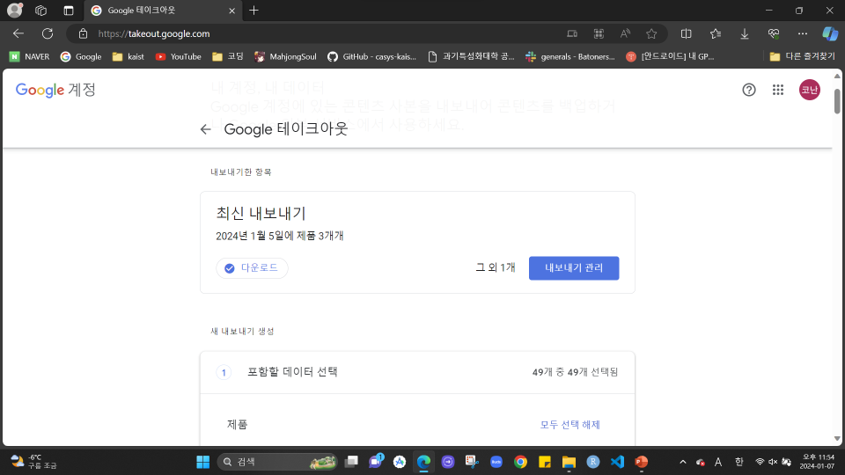
\includegraphics[width=\textwidth]{Google_takeout_1.png}    
  \end{figure}
  \subsection{Google\_takeout}
  모두 선택 해제를 한다.
  \begin{figure}[H]
    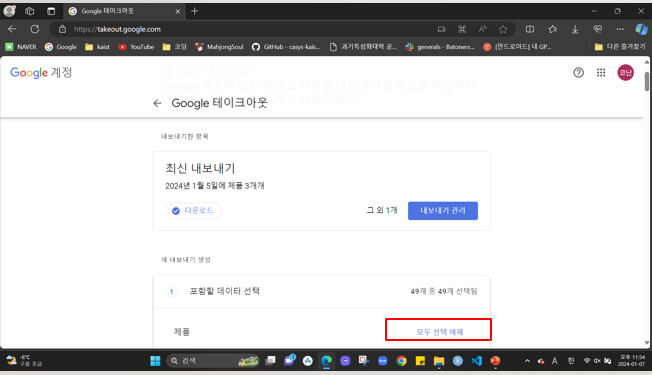
\includegraphics[width=\textwidth]{Google_takeout_2.png}
  \end{figure}
  \subsection{Google\_takeout}
  포함할 데이터선택에서 위치 기록, 지도, 지도(내 장소)를 선택한다.
  \begin{figure}[H]
    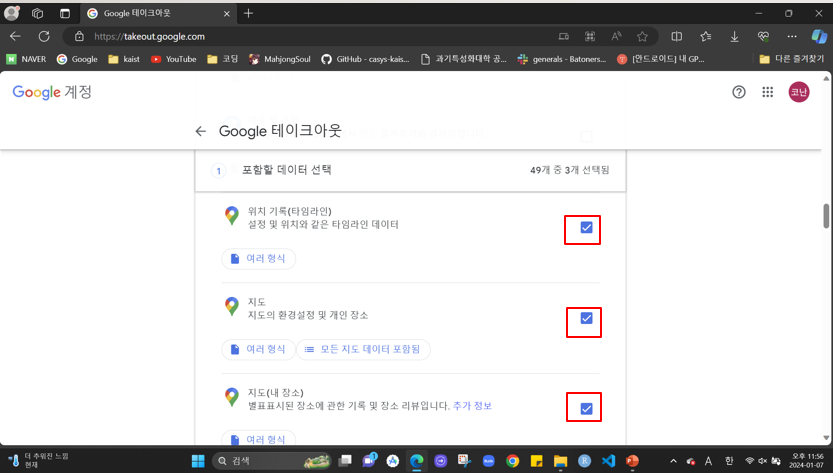
\includegraphics[width=\textwidth]{Google_takeout_3.png}
  \end{figure}      
  \subsection{Google\_takeout}
  하단의 다음 단계를 클릭한다.
  \begin{figure}[H]
    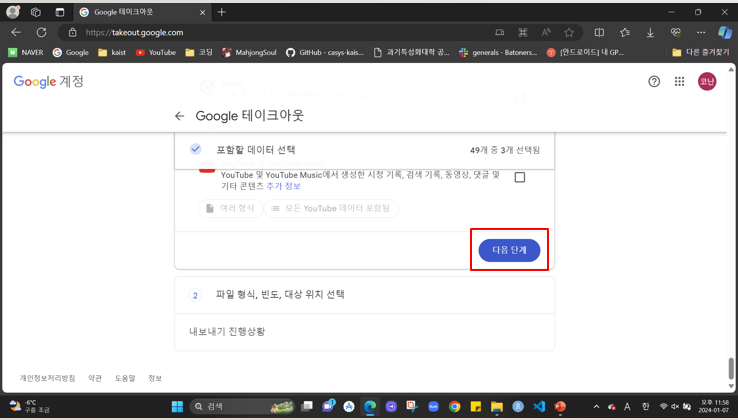
\includegraphics[width=\textwidth]{Google_takeout_4.png}
  \end{figure}      
  \subsection{Google\_takeout}
  하단의 내보내기 생성을 클릭한다.
  \begin{figure}[H]
    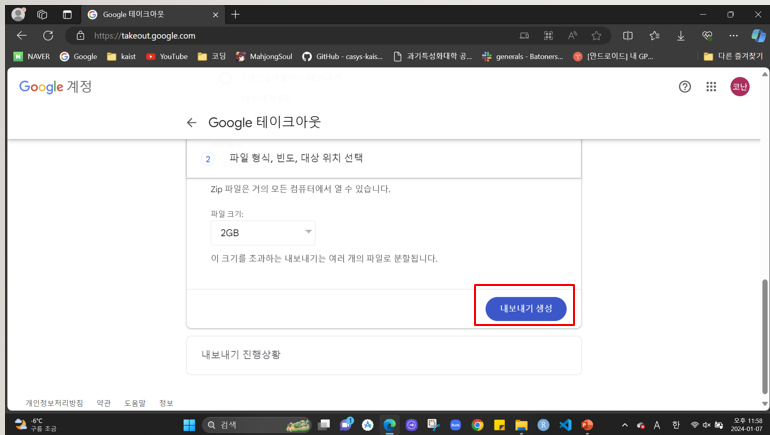
\includegraphics[width=\textwidth]{Google_takeout_5.png}
  \end{figure}     
  \subsection{Google\_takeout}
  G-mail에 들어가 Google 테이크아웃 메일이 온 것을 확인한다.
  \begin{figure}[H]
    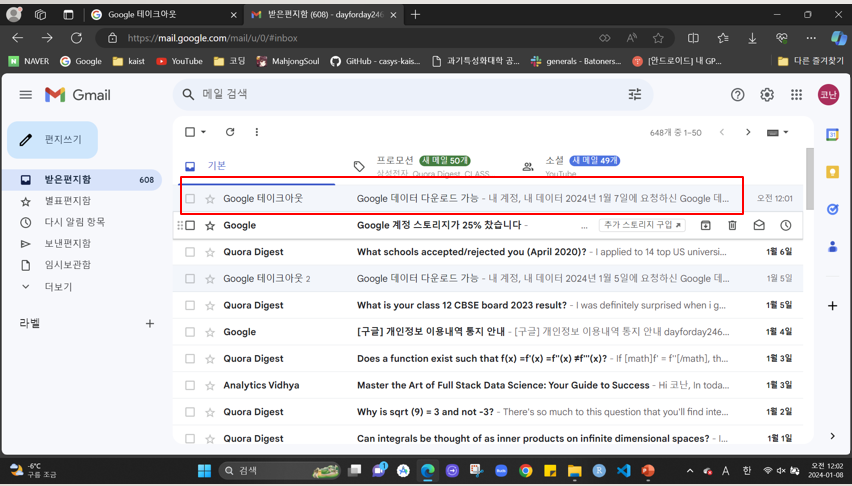
\includegraphics[width=\textwidth]{Google_takeout_6.png}
  \end{figure}
  \subsection{Google\_takeout}
  메일 속 파일을 다운로드한다.
  \begin{figure}[H]
    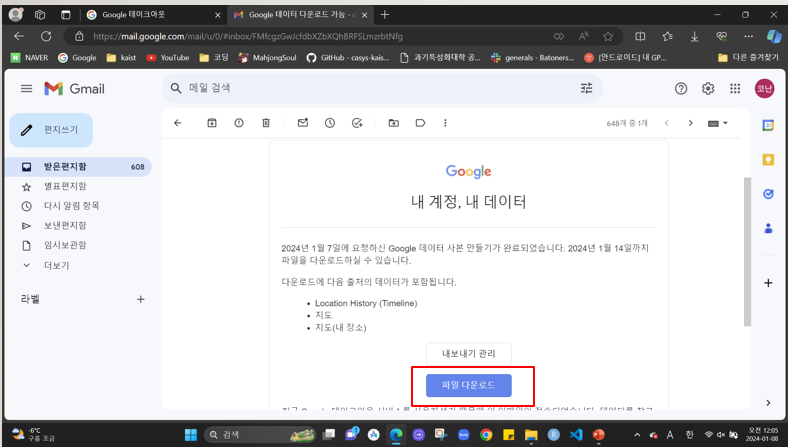
\includegraphics[width=\textwidth]{Google_takeout_7.png}
  \end{figure}
  \subsection{Google\_takeout}
  압축해제 후, Takeout\textbackslash Location History(Timeline)\textbackslash Records.json가 있는지 확인한다.
  \begin{figure}[H]
    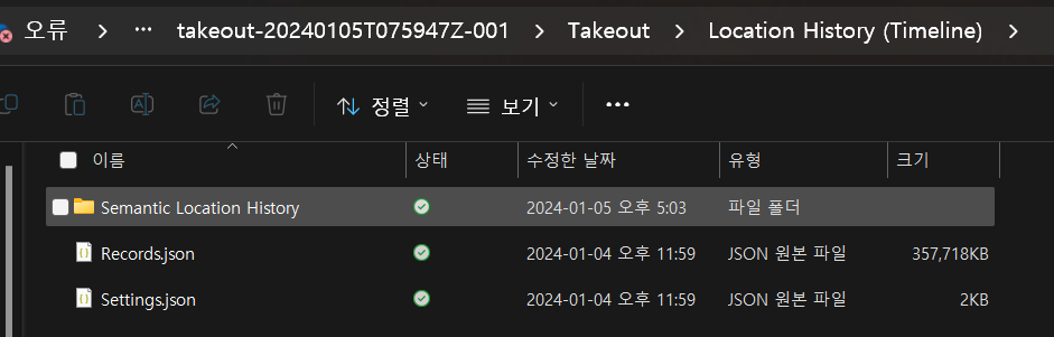
\includegraphics[width=\textwidth]{Google_takeout_8.png}
  \end{figure}

  \section{사용법}
  Records.json를 GPS\_dataload파일에 넣고, GPS\_dataload.py를 실행시켜 data.csv파일을 생성한다.
  \begin{figure}[H]
    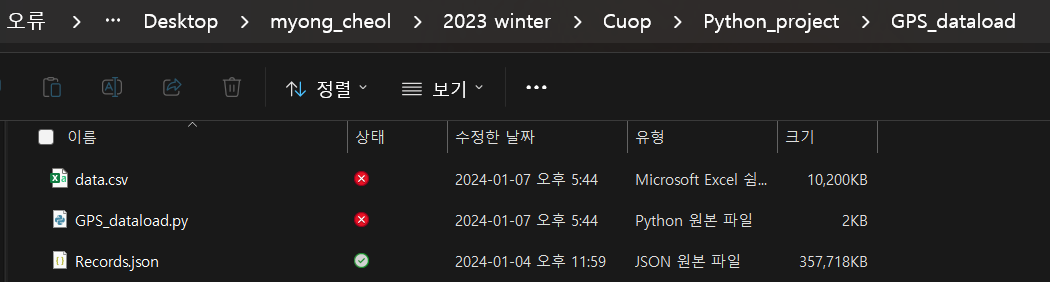
\includegraphics[width=\textwidth]{Google_takeout_9.png}
  \end{figure}

  \section{코드설명}
  먼저, Records.json 파일을 열어 읽고 닫습니다.
  \begin{python}[label={GPS_dataload_1}]
    root_dir = os.path.dirname(os.path.abspath(__file__))
    json_dir = os.path.join(root_dir, "Records.json")
    f = open(json_dir)
    data = json.load(f)
    f.close()
  \end{python}
  Records.json에서 latitudeE7, longitudeE7, timestamp를 읽습니다.
  \begin{python}[label={GPS_dataload_1}]
    location_data = data["locations"]

    df = pd.DataFrame(
        {
            "latitude": [entry["latitudeE7"] for entry in location_data],
            "longitude": [entry["longitudeE7"] for entry in location_data],
            "time": [entry["timestamp"] for entry in location_data],
        }
    )
  \end{python}
  읽은 데이터로 latitude, longitude, obtained\_at를 만듭니다. create\_at은 프로그램을 돌리는 시각을 넣는 것으로 합니다.
  \begin{python}[label={GPS_dataload_3}]
    df["obtained_at"] = pd.to_datetime(df["time"].str[:19], format="%Y-%m-%dT%H:%M:%S")
    df["created_at"] = pd.Timestamp.now()
    df["created_at"] = df["created_at"].dt.strftime("%Y-%m-%d %H:%M:%S")
    df = df.drop(columns="time")

    df["latitude"] = df["latitude"] / (10**7)
    df["longitude"] = df["longitude"] / (10**7)    
  \end{python}
  같은 폴더에 data.csv로 저장합니다.
  \begin{python}[label=GPS_dataload_4]
    df.to_csv(os.path.join(root_dir, "data.csv"), index=False)
  \end{python}

  \chapter{Label\_dataload}
  \setcounter{section}{0}
  \section{데이터 수집}
  GPS\_dataload에서 사용한 Takeout 파일을 그대로 사용하여 사용자에게 의미가 있는 장소들(집, 직장, 학교 등)에 대한 정보를 얻습니다.
  Takeout\textbackslash Maps\textbackslash My labeled places\textbackslash Labeled places.json파일을 확인하여 라벨이 지정된 장소들을 확인합니다.
  \begin{figure}[H]
    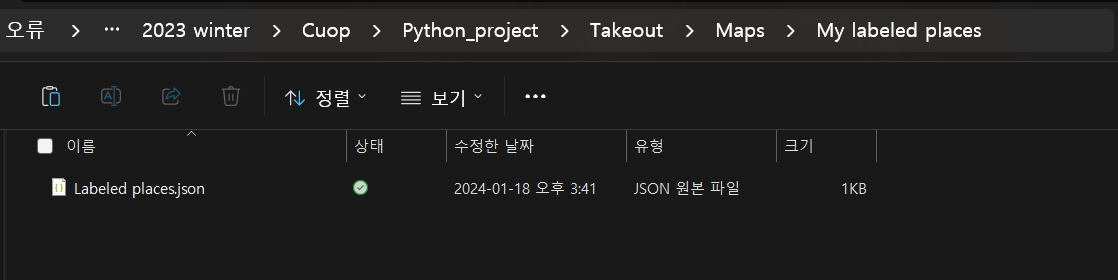
\includegraphics[width=\textwidth]{Label_dataload_1.png}
  \end{figure}
  \section{사용법}
  Labeled places.json 파일을 Label\_dataload파일에 넣고 Label\_dataload.py를 실행하여 label.csv파일을 생성합니다.
  \begin{figure}[H]
    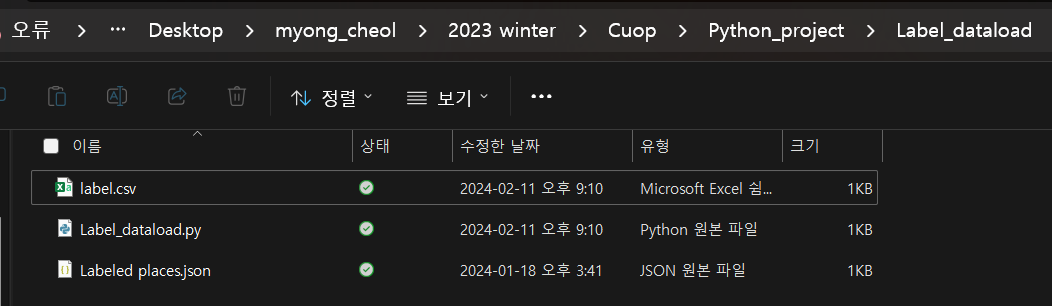
\includegraphics[width=\textwidth]{Label_dataload_2.png}
  \end{figure}

  \section{코드 설명}
  먼저, Labeled places.json파일을 열어 읽고 닫습니다.
  \begin{python}[label={Label_dataload_1}]
    root_dir = os.path.dirname(os.path.abspath(__file__))
    json_dir = os.path.join(root_dir, "Labeled places.json")
    f = open(json_dir)
    data = json.load(f)
    f.close()
  \end{python}
  Labeled places.json에서 geometry의 coordinates에 저장된 장소의 위도, 경도와 properties의 name에 저장된 장소의 이름을 읽습니다.
  그 후, 이것을 latitude, longitude, name의 컬럼으로 데이터프레임에 저장합니다.
  \begin{python}[label={Label_dataload_2}]
    label_data = data["features"]

    df = pd.DataFrame(
        {
            "latitude": [entry["geometry"]["coordinates"][1] for entry in label_data],
            "longitude": [entry["geometry"]["coordinates"][0] for entry in label_data],
            "name": [entry["properties"]["name"] for entry in label_data],
        }
    )
      \end{python}
  같은 폴더에 label.csv로 저장합니다.
  \begin{python}[label={Label_dataload_3}]
    df.to_csv(os.path.join(root_dir, "label.csv"), index=False)
  \end{python}

  \chapter{GPS\_preprocess}
  \setcounter{section}{0}
  \section{데이터 수집}
  GPS\_preprocess에서 사용할 데이터는 Google takeout에서 가져온 raw data입니다.
  GPS\_dataload에서 data.csv를 GPS\_preprocess\textbackslash Data로 복사합니다.
  \begin{figure}[H]
    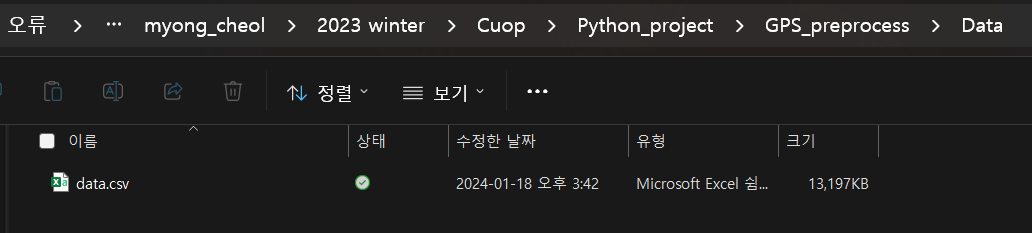
\includegraphics[width=\textwidth]{GPS_preprocess_1.png}
  \end{figure}

  \section{사용법}
  GPS\_preprocess파일에서 GPS\_preprocess.py를 실행하면 Filtered\_data에 data\_cleaned.csv와 data\_smoothed.csv가 생성됩니다.
  GPS\_preprocess.py는 GPS\_clean.py를 실행시켜 data.csv로부터 data\_cleaned.csv를 만들어 냅니다.
  그 후, GPS\_smoothed.py를 실행시켜 data\_smoothed.csv를 만들게 됩니다.
  \begin{figure}[H]
    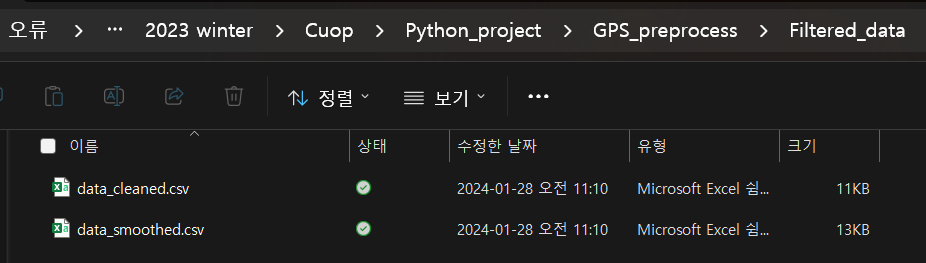
\includegraphics[width=\textwidth]{GPS_preprocess_2.png}
  \end{figure}

  \section{GPS\_clean.py}
  \subsection{이론 설명}
  본 코드는 Schussler\cite{Schussler}를 참고하여 만들었습니다.
  논문에서는 GPS sudden position jump가 일어나면 갑자기 속도가 비정상적인 값이 나온다고 했습니다.
  따라서 불가능한 속도를 가진 점들을 GPS sudden position jump로 보고 제거하여 data clean을 진행했습니다.
  그러나 제가 가진 데이터에서는 그런 경향성이 나타나지 않았습니다.
  제 1월 17일 데이터를 가지고 시간에 따른 이동 거리와 속도에 대한 그래프를 그려봤습니다.(집에서 충남대학교 Tipstown으로 출퇴근한 데이터입니다.)
  새벽 4시와 오전 11시에 실제로 움직이지 않았지만, 큰 움직임이 관측됩니다.
  그 때의 속도를 구해보니, 정상적인 움직임을 보일 때와 비교할 때, 큰 차이가 있지 않았습니다.
  \begin{figure}[H]
    \caption{GPS Path와 시간에 따른 이동거리, 속도 그래프}
    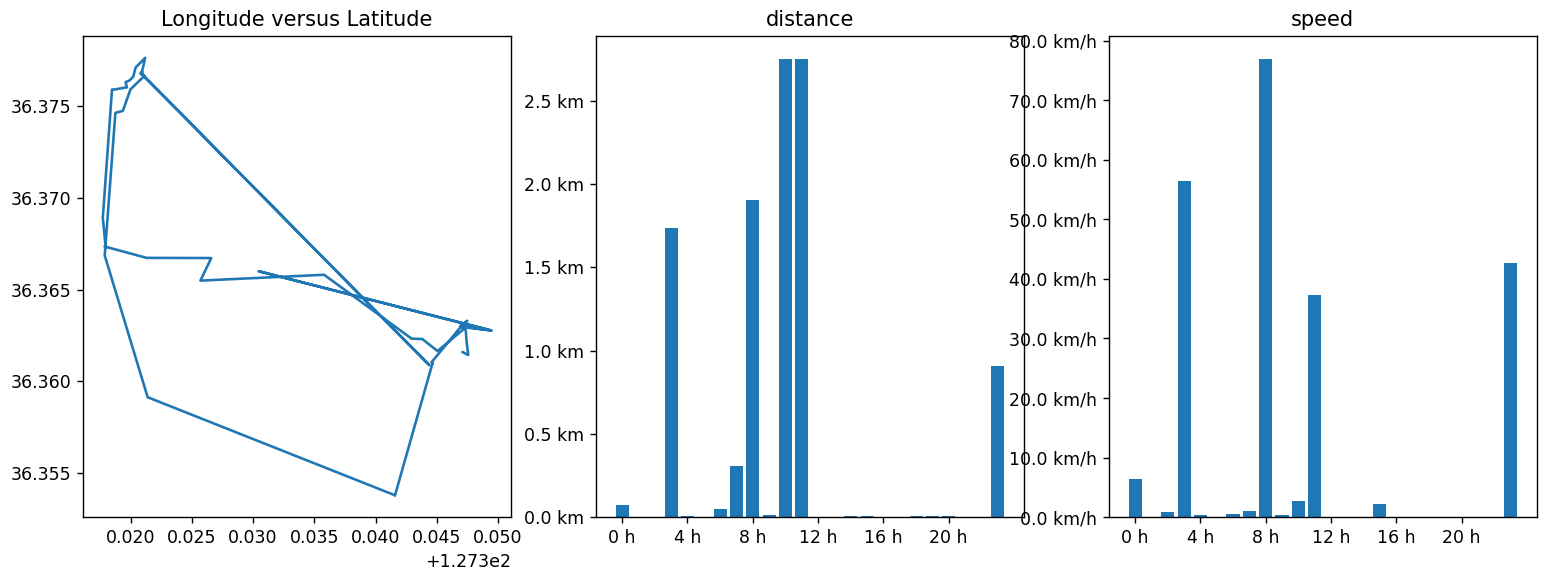
\includegraphics[width=\textwidth]{GPS_preprocess_3.png}
  \end{figure}
  따라서 논문과는 다른 방법으로 data clean을 구현해야겠다고 생각했습니다.\newline
  제 알고리즘의 구성은 다음과 같습니다.
  \paragraph{GPS\_clean 알고리즘}
  \begin{enumerate}
    \item 하버사인 공식(harversine formula)을 사용하여 연속된 두 데이터 사이의 이동거리를 구합니다.
    \item distance\_threshold보다 더 많이 움직인 점들을 기준으로 데이터를 잘라 $segment_1,\ldots,segment_n$를 만듭니다.
    \item 각 segment의 평균 위치인 $P_i$를 구합니다.
    \item 만약 $segment_i$가 jump\_threshold 이하의 데이터 개수를 가지고, $P_{i-1}$과 $P_{i+1}$ 사이의 거리가 same\_place\_threshold보다 작으면 GPS sudden position jump로 인식합니다.
  \end{enumerate}
  distance\_threshold, jump\_threshold, same\_place\_threshold를 적당히 조절하여 주어진 데이터에 적합한 값을 찾아야 합니다.
  제 1월 17일의 데이터에서는 $distance\_threshold=0.75,jump\_threshold=3,same\_place\_threshold=0.3$을 사용하여 진행했습니다.
  distance\_threshold와 same\_place\_threshold의 단위는 Km입니다. 
  \begin{figure}[H]
    \caption{Before and After of cleaning}
    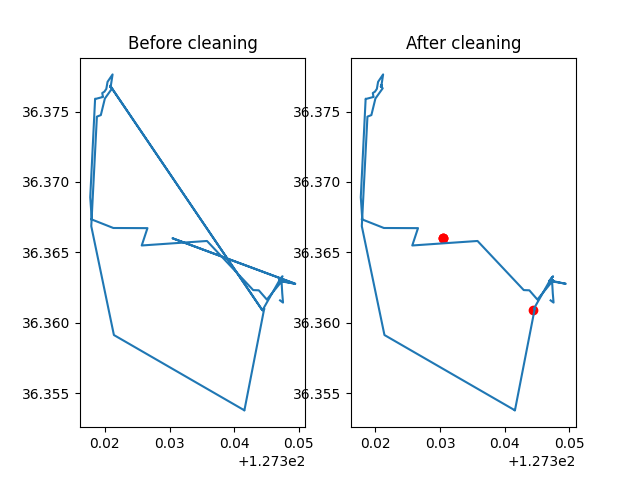
\includegraphics[width=\textwidth]{GPS_preprocess_4.png}
  \end{figure}

  \subsection{코드 설명}
  먼저, data.csv를 읽습니다.
  \begin{python}[label={GPS_clean_1}]
    root_dir = os.path.dirname(os.path.abspath(__file__))
    data_dir = os.path.join(os.path.join(root_dir, "Data"), "data.csv")
    data = pd.read_csv(data_dir)
    data["obtained_at"] = pd.to_datetime(data["obtained_at"])
    data["created_at"] = pd.to_datetime(data["created_at"])
  \end{python}
  2024년 1월 17일 데이터를 선택합니다.
  \begin{python}[label={GPS_clean_2}]
    data = data[
      (data["obtained_at"].dt.year == 2024)
      & (data["obtained_at"].dt.month == 1)
      & (data["obtained_at"].dt.day == 17)
    ]
  \end{python}
  하버사인 공식을 사용하기 위해, 공식이 구현되어 있는 FeatureMaker 클래스의 인스턴스를 생성합니다.
  (FeatureMaker 클래스는 GPS\_feature에서 소개할 예정입니다.)
  \begin{python}[label={GPS_clean_3}]
    featuremaker = FeatureMaker()
  \end{python}
  하버사인 공식을 이용해 이동거리를 구합니다. 이 때, 마지막 for-loop는 제외합니다.
  (하버사인 공식을 이용할 때, i번째 데이터와 i+1번째 데이터를 사용하기 때문입니다.)
  \begin{python}[label={GPS_clean_4}]
    distance = list()
    for i in range(data.shape[0]):
        if i == data.shape[0] - 1:
            break
        distance.append(
            featuremaker.harversine(data.iloc[i], data.iloc[i + 1])
        )
  \end{python}
  distance\_threshold 이상의 거리를 움직인 데이터를 기준으로 원본 데이터를 잘라 segments 리스트에 저장합니다.
  \begin{python}[label={GPS_clean_5}]
    segments = list()
    i = 0
    segment = []
    while i < len(distance):
        if distance[i] > distance_threshold:
            segments.append(segment)
            segment = []
        segment.append(i)
        i += 1
    segment.append(i)
    segments.append(segment)
  \end{python}
  각 segment별로, 그 평균 위치를 구해 segments\_mean에 저장합니다.
  \begin{python}[label={GPS_clean_6}]
    segments_mean = [
      data[["longitude", "latitude"]].iloc[segment].mean()
      for segment in segments
    ]
  \end{python}
  만약 i번째 segment가 jump\_threshold 이하의 데이터 개수를 가지고, i-1번째 segment의 평균 위치와 i+1번째 segment의 평균 위치 사이의 거리가 same\_place\_threshold 이하이면 jump 리스트에 i를 넣습니다.
  즉, jumps 리스트에는 GPS sudden position jump로 인식된 segment들의 index가 저장됩니다.
  \begin{python}[label={GPS_clean_7}]
    jumps = list()
    for i in range(1, len(segments_mean) - 1):
        if (
            len(segments[i]) <= jump_threshold
            and featuremaker.harversine(segments_mean[i - 1], segments_mean[i + 1])
            < same_place_threshold
        ):
            jumps.append(i)
  \end{python}
  jump 리스트에 담긴 segment의 index를 토대로 GPS sudden position jump로 인식된 segment들을 제거합니다.
  jump\_index는 인식된 segment들을 구성하고 있는 데이터의 index를 나타냅니다.
  \begin{python}[label={GPS_clean_8}]
    jump_index = np.array([])
    if len(jumps) > 0:
        jump_index = np.concatenate([segments[jump] for jump in jumps])
        jump_index += 1
        data_filtered = pd.DataFrame(np.delete(data, jump_index, axis=0))
        data_filtered.columns = data.columns
    else:
        data_filtered = data.copy()
  \end{python}
  cleaning을 마친 데이터를 Filtered\_data 폴더에 data\_cleaned.csv로 저장합니다.
  \begin{python}[label={GPS_clean_9}]
    filtered_dir = os.path.join(root_dir, "Filtered_data")
    data_filtered.to_csv(
        os.path.join(filtered_dir, "data_cleaned.csv"), index=False
    )
  \end{python}

  \section{GPS\_smooth.py}
  \subsection{이론 설명}
  본 코드는 Schussler\cite{Schussler}를 참고하여 만들었습니다. 논문에서 사용한 Gaussian kernel smoothing을 사용했습니다.
  \begin{definition}[Gaussian kernel smoothing]
    주변 관측 데이터의 가중 평균으로 관측치를 추정하는 기법을 kernel smoothing이라고 한다.
    Gaussian kernel smoothing의 경우 가중치를 Gaussian 함수에 추정하는 관측치와 주변 관측치 사이의 거리를 넣어 정한다. 
  \end{definition}
  즉, 원본 데이터가 $G=\{g_1,\ldots,g_n\}$로 주어져 있고, $f\sim n(0,\sigma^2)$이면,
  smoothing을 거친 데이터 $G'=\{g_1',\ldots,g_n'\}$는 $g_i'=\sum_{k=1}^n{f(D(g_i,g_k))g_k}/\sum_{k=1}^n{f(D(g_i,g_k))}$이다.
  이 때, $D$는 거리 함수로 보통 유클리디안(Euclidean)을 쓴다. $g_k$가 가중치 $f(D(g_i,g_k))/\sum_{k=1}^n{f(D(g_i,g_k))}$를 가지고 있음을 볼 수 있다.
  만약, $g_k$가 $g_i$와 가깝다면 큰 영향을 줄 것이고, 아니라면 거의 영향을 주지 못한다. 따라서 전후의 상황을 고려해 매끄럽게 만들어준다.\newline
  $\sigma$의 경우, 데이터를 보고 적절히 조절해야 한다. 본 프로젝트는 $\sigma=90$을 사용했다. $\sigma$의 단위는 초이다.
  $\sigma$가 작으면 효과가 미미할 것이고, 크다면 과도하게 데이터를 변형할 위험이 있다.
  다음은 $\sigma=60$일 때와 $\sigma=120$일 때, smoothing 전후를 비교한 그림입니다.
  \begin{figure}[H]
    \centering
    \begin{subfigure}[b]{0.5\textwidth}
      \centering
      \subcaption{$\sigma=60$}
      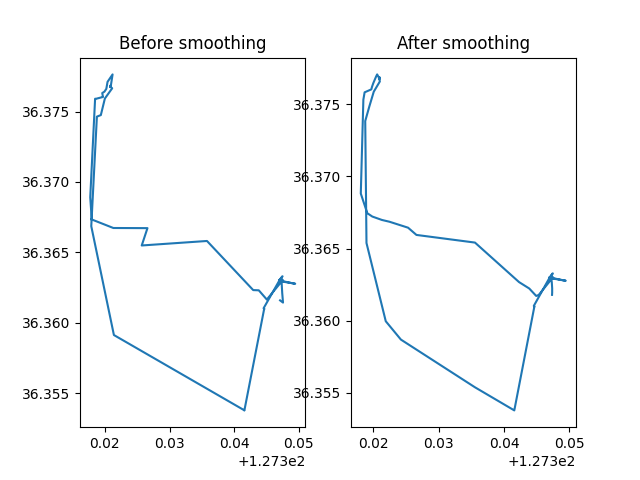
\includegraphics[width=\textwidth]{GPS_preprocess_5.png}        
    \end{subfigure}%
    \begin{subfigure}[b]{0.5\textwidth}
      \centering
      \subcaption{$\sigma=120$}
      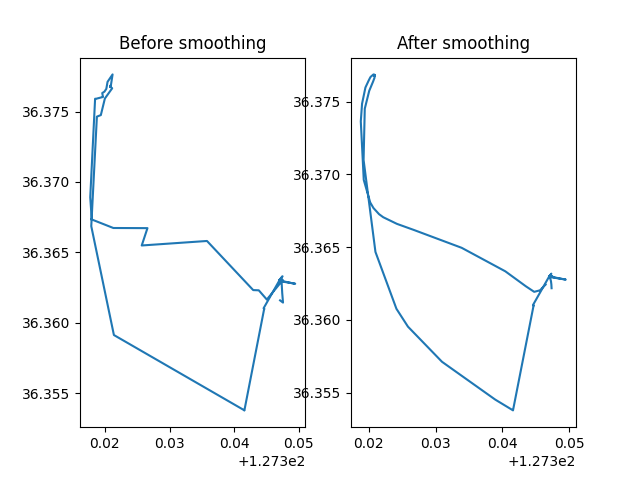
\includegraphics[width=\textwidth]{GPS_preprocess_6.png}
    \end{subfigure}
    \caption{smoothing 전후 비교}
  \end{figure}
    

  \subsection{코드 설명}
  먼저, data\_cleaned.csv를 읽습니다.
  \begin{python}[label={GPS_smooth_1}]
    root_dir = os.path.dirname(os.path.abspath(__file__))
    data_dir = os.path.join(os.path.join(root_dir, "Filtered_data"), "data_cleaned.csv")
    data = pd.read_csv(data_dir)
    data["obtained_at"] = pd.to_datetime(data["obtained_at"])
    data["created_at"] = pd.to_datetime(data["created_at"])
  \end{python}
  읽은 데이터로 Gaussian 가중치를 생성합니다. 거리는 시간 차이로 설정했고, $\sigma=90$입니다.
  Gaussian함수의 지수함수에 붙은 계수는 가중치를 구하며 사라지니 생략했습니다.
  Gaussian[i]에는 i번째 데이터의 가중치가 들어있습니다.
  \begin{python}[label={GPS_smooth_2}]
    diff_time = np.array(
        [data["obtained_at"] - t for t in data["obtained_at"]]
    ) / pd.Timedelta(seconds=sigma)
    Gaussian = np.exp(-(diff_time**2) / 2)
    Gaussian = np.array([i / np.sum(i) for i in Gaussian])
  \end{python}
  Gaussian 가중치를 이용하여 longitude의 가중 평균을 구해 longitude를 smoothing합니다.
  가중 평균은 가중치와 longitude의 내적과 같음으로, 행렬곱을 사용해서 구했습니다.
  \begin{python}[label={GPS_smooth_3}]
    data["longitude"] = np.array(
      [np.matmul(Gaussian[i], data["longitude"]) for i in range(len(Gaussian))]
    )
  \end{python}
  latitude에도 똑같이 적용합니다.
  \begin{python}[label={GPS_smooth_4}]
    data["latitude"] = np.array(
      [np.matmul(Gaussian[i], data["latitude"]) for i in range(len(Gaussian))]
    )
  \end{python}
  Filtered\_data폴더에 data\_smoothed.csv로 smoothing한 데이터를 저장합니다.
  \begin{python}[label={GPS_smooth_5}]
    filtered_dir = os.path.join(root_dir, "Filtered_data")
    data.to_csv(os.path.join(filtered_dir, "data_smoothed.csv"), index=False)
  \end{python}

  \chapter{GPS\_clustering}
  \setcounter{section}{0}
  \section{데이터 수집}
  다양한 상황을 가정하고 clustering 알고리즘을 평가하기 위해, 실제 GPS 데이터를 쓰지 않고 numpy에서 제공하는 메소드를 사용하기로 했습니다.
  따라서 따로 데이터 수집이 필요하지 않습니다.

  \section{모듈: GPS\_clustering.py}
  modules 폴더를 열어보면 아래와 같이 GPS\_clustering.py와 GPS\_feature.py의 두 모듈이 있는 것을 확인할 수 있습니다.
  GPS\_clustering.py는 ClusterGenerator, Classifier의 두 클래스로 구성되어 있습니다.
  \begin{figure}[H]
    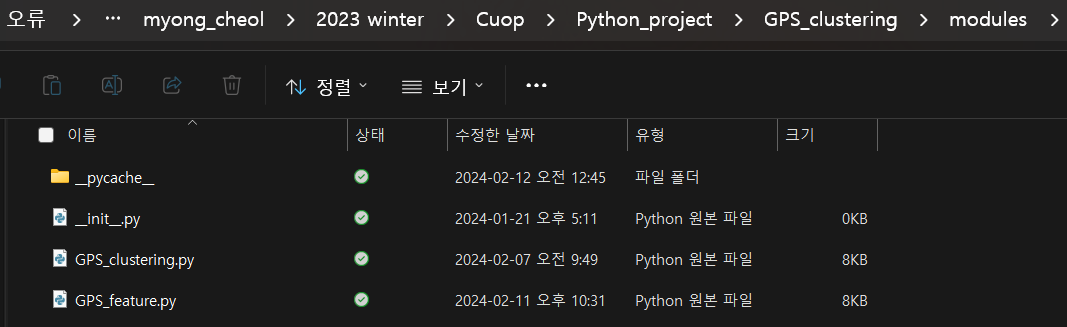
\includegraphics[width=\textwidth]{GPS_clustering_1.png}
  \end{figure}

  \subsection{클래스: ClusterGenerator}
  ClusterGenerator 클래스의 구조는 다음과 같습니다.
  \dirtree{%
  .0 GPS\_clustering.py.
  .1 class: ClusterGenerator.
  .2 method: self.\_\_init\_\_.
  .2 method: self.generate\_cluster.
  .2 method: self.plot\_clusters.
  .2 method: self.show\_clusters.
  .2 method: self.save\_clusters.
  .1 class: Classifier.
  }
  ClusterGenerator는 이름대로 클러스터를 만들기 위한 클래스입니다.
  self.\_\_init\_\_에서는 seed를 설정할 수 있습니다. seed 정해 결과를 재현할 수 있습니다.
  self.generate\_cluster에서는 multivariate normal의 평균과 분산행렬을 받아 하나의 클러스터를 만들 수 있습니다.(GPS 데이터를 다루기 때문에 이차원이어야 합니다.)
  self.plot\_clusters는 self.show\_clusters와 self.save\_clusters를 보조하는 함수입니다.
  만약 save\_path argument가 None이라면 self.show\_clusters 함수가 호출된 것으로 인식하고 클러스터들을 그립니다.
  아니면 self.save\_clusters 함수가 호출된 것으로 인식하고 클러스터들을 그린 그림을 save\_path에 저장합니다.
  clusters argument는 리스트이며 한 원소에 한 클러스터의 데이터들이 들어 있습니다. 
  자세한 코드 설명은 본 문서의 목적과 맞지 않는 것 같아, 파이썬의 numpy, matplotlib 모듈을 참조하는 것으로 넘어가겠습니다.

  \subsection{클래스: Classifier}
  Classifier 클래스의 구조는 다음과 같습니다.
  \dirtree{%
  .0 GPS\_clustering.py.
  .1 class: ClusterGenerator.
  .1 class: Classifier.
  .2 method: self.\_\_init\_\_.
  .2 method: self.k\_mean.
  .2 method: self.DBSCAN.
  .2 method: self.\_\_extend\_cluster.
  .2 method: self.adaptive\_k\_mean.
  .2 method: self.neighbor.
  .2 method: self.plot\_clusters.
  .2 method: self.show\_clusters.
  .2 method: self.save\_clusters.
  }
  Classifier는 주어진 데이터를 clustering하는 것을 목표로 하는 클래스입니다.
  self.\_\_init\_\_의 경우, ClusterGenerator 클래스처럼 seed를 받고 있습니다.
  self.k\_mean에서는 k-mean clustering 알고리즘을 사용하여 주어진 데이터를 clustering합니다.
  self.DBSCAN에서는 DBSCAN clustering 알고리즘을 사용하여 주어진 데이터를 clustering합니다.
  self.\_\_extend\_cluster는 self.DBSCAN의 보조함수로 사용됩니다.
  self.adaptive\_k\_mean에서는 adaptive-k-mean clustering 알고리즘을 사용하여 주어진 데이터를 clustering합니다.
  self.neighbor에서는 주어진 data에서 point와의 거리가 rad 이하인 점들을 고르는 clustering을 합니다.
  나머지는 ClusterGenerator와 같습니다. 다만, clusters 대신 data와 label을 받습니다.
  label은 clustering한 결과, 데이터가 어떤 cluster에 할당되었는지 나타내는 리스트입니다.
  예를 들어, data에 3개의 데이터가 있고 각 데이터가 다른 cluster에 할당되었다면 label은 [0,1,2]입니다.
  클러스터의 index는 0부터 시작하며 -1은 할당되지 않음을 의미합니다.

  \section{self.k\_mean}
  \subsection{이론 설명}
  k-mean clustering 알고리즘은 가장 보편적으로 사용되는 clustering 알고리즘 중 하나이며 많은 variation이 존재한다.
  k-mean clustering 알고리즘은 다음과 같은 단계로 수행된다.
  \paragraph{k-mean clustering 알고리즘}
  \begin{enumerate}
    \item 먼저, cluster 개수인 k를 정한다.
    \item 각 데이터 $g_i$를 랜덤으로 어느 하나의 cluster에 할당한다. 예를 들어 $g_i$가 j번째 cluster에 포함되면, $f(g_i)=j$입니다.
    \item $C_j=\{g_i|f(g_i)=j\}$의 평균 위치로 j번째 cluster의 중심인 $centroid_j$를 구합니다.
    \item 각 데이터를 가장 가까운 중심의 cluster로 재할당합니다.
    \item 앞의 두 과정을 iteration번 반복합니다.
  \end{enumerate}
  가장 가까운 중심을 찾을 때 사용하는 거리의 종류에 따라 알고리즘을 부르는 이름이 다릅니다. k-mean clustering 알고리즘은 유클리디안(Euclidean)을 사용합니다.
  과정을 반복함에 따라, 점차 clustering이 어느 한 상태로 수렴하는 것을 볼 수 있습니다.

  \subsection{예시: K\_mean.py}
  다음은 클러스터1($\mu_1=\begin{pmatrix}1\\1\end{pmatrix},\sigma_1=\begin{pmatrix}1 & 0 \\ 0 & 1\end{pmatrix}$)과
  클러스터2($\mu_2=\begin{pmatrix}-1\\-1\end{pmatrix},\sigma_2=\begin{pmatrix}1 & 0 \\ 0 & 1\end{pmatrix}$)에서
  각각 데이터 50개씩을 만들어 $k=2,iteration=10$으로 k-mean clustering을 해본 결과입니다.
  \begin{figure}[H]
    \begin{subfigure}[b]{.5\textwidth}
      \centering
      \subcaption{Before k-mean clustering}
      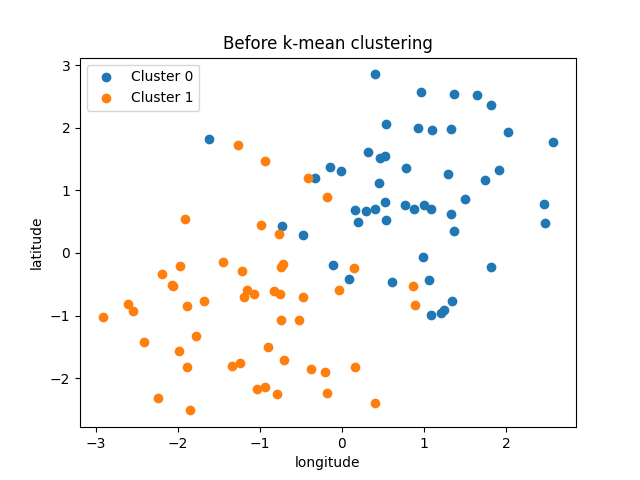
\includegraphics[width=\textwidth]{GPS_clustering_2.png}
    \end{subfigure}%
    \begin{subfigure}[b]{.5\textwidth}
      \centering
      \subcaption{After k-mean clustering}
      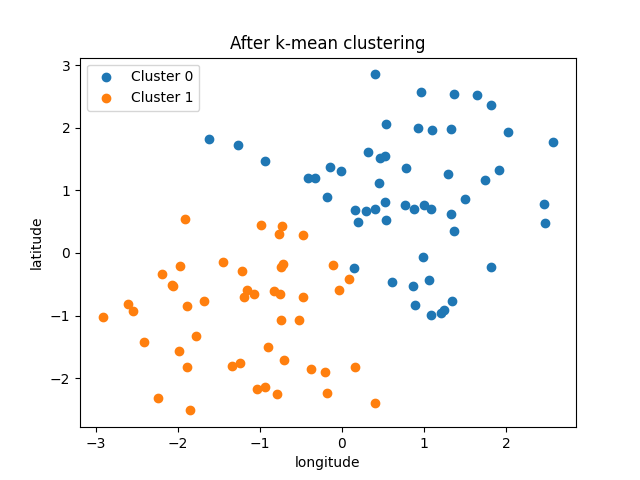
\includegraphics[width=\textwidth]{GPS_clustering_3.png}      
    \end{subfigure}
    \caption{k-mean 예시}
  \end{figure}
  원본 데이터의 경우 클러스터1과 클러스터2가 산재된 곳이 있지만, k-mean clustering을 적용한 후엔 완벽히 분리되는 것을 볼 수 있습니다.
  이것은 k-mean clustering 알고리즘이 centroid와의 거리를 기준으로 clustering을 하기 때문입니다.
  따라서 k-mean clustering은 산재된 데이터를 완벽히 분류할 수는 없습니다.

  \subsection{코드 설명}
  \subsubsection{Classifier.k\_mean}
  Label은 데이터가 어떤 cluster에 할당되었는지 알려주는 리스트입니다.
  먼저, Label을 랜덤한 값으로 초기화합니다. 그리고 빈 centroid 리스트도 만듭니다.
  \begin{python}[label={GPS_clustering_1}]
    label = np.random.choice(k, data.size // 2, replace=True)
    centroid = [np.array([]) for _ in range(k)]
  \end{python}
  랜덤하게 할당된 Label을 가지고 centroid 리스트를 채워줍니다.
  \begin{python}[label={GPS_clustering_2}]
    for i in range(k):
      centroid[i] = np.mean(data[label == i], axis=0)
  \end{python}
  데이터와 centorid 사이의 거리를 구해 distance에 저장합니다. 그 후, 가장 가까운 centroid에 따라 Label을 재할당합니다.
  그리고 재할당된 Label을 이용해 centroid를 갱신합니다. 이 과정을 iteration번 반복합니다.
  \begin{python}[label={GPS_clustering_3}]
    for _ in range(iteration):
      distances = np.array([np.linalg.norm(data - c, axis=1) for c in centroid])
      label = np.argmin(distances, axis=0)
      for i in range(k):
        centroid[i] = np.mean(data[label == i], axis=0)
  \end{python}
  완성된 Label을 반환합니다.
  \begin{python}[label={GPS_clustering_4}]
    return Label
  \end{python}

  \section{self.DBSCAN}
  \subsection{이론 설명}
  Sohrab\cite{Sohrab}에서 나온 피쳐분석을 하기 위해 clustering을 하는 중, 의문이 하나 생겼다.
  \emph{"k-mean clustering 알고리즘은 클러스터의 개수인 k를 알아야한다."}
  우리는 일반적으로 클러스터의 개수를 알지 못한다. 따라서 다른 종류의 알고리즘이 필요해 보였다.
  김소정\cite{김소정}에서는 DBSCAN clustering을 이용하여 오차를 보정하는 방법에 대해 설명하고 있다.
  DBSCAN clustering 알고리즘은 밀도 기반의 clustering 알고리즘이다.
  어떤 반경(radious)에 특정 개수(threshold) 이상의 데이터가 존재한다면 클러스터로 취급하고, 그 보다 희박하게 데이터가 있다면 전부 노이즈로 취급한다.
  사전에 클러스터의 개수를 정해주지 않고, 밀도에 대한 정보만 넣으면 알아서 클러스터링을 한다는 점에서 GPS 데이터의 클러스터링에 적합해보였다.
  \paragraph{DBSCAN clustering 알고리즘}
  \begin{enumerate}
    \item 어떤 데이터가 core data인지 noise인지 구분합니다. 기준은 데이터 주변 rad이하의 반경에, thres이상의 데이터 개수가 있는지 입니다.
    \item core data에서 아무 데이터 하나를 잡고 빈 클러스터에 할당합니다. 반경 rad안의 다른 데이터를 그 클러스터에 할당 후, 할당된 데이터에서 반복적으로 더 이상 변화가 없을 때까지 클러스터를 확장합니다.
    \item 만약, 할당되지 않은 core data가 클러스터 확장 후에도 남았다면 모든 core data가 할당이 될 때까지 앞의 과정을 반복합니다.
    \item noise의 경우, core data 할당 후, 반경 rad안의 가장 가까운 데이터의 클러스터로 할당합니다. 만약 반경 rad안에 데이터가 없다면 할당하지 않습니다.
  \end{enumerate}
  DBSCAN clustering의 장점은 클러스터의 개수를 미리 정하지 않는다는 점과 클러스터로 할당하지 않은 noise도 생긴다는 점입니다.
  GPS 데이터는 장소에 머무르는 경우도 있지만, 이동하는 중인 데이터도 있기 때문에 그런 점들은 클러스터로 할당하지 않아야 합니다.
  따라서 이런 목적에서 DBSCAN clustering은 최적의 알고리즘입니다.

  \subsection{예시: DBSCAN.py}
  다음은 클러스터1($\mu_1=\begin{pmatrix}10\\10\end{pmatrix},\sigma_1=\begin{pmatrix}10&5\\5&10\end{pmatrix}$)과
  클러스터2($\mu_2=\begin{pmatrix}-10\\-10\end{pmatrix},\sigma_2=\begin{pmatrix}10&-5\\-5&10\end{pmatrix}$)에서
  각각 데이터를 50개씩 만들어, $rad=4,thres=3$으로 DBSCAN clustering을 해본 결과입니다.
  \begin{figure}[H]
    \begin{subfigure}[b]{.5\textwidth}
      \centering
      \caption{Before DBSCAN clustering}
      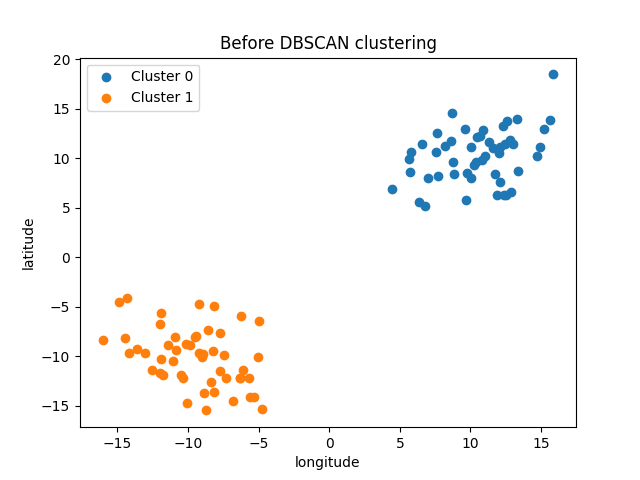
\includegraphics[width=\textwidth]{GPS_clustering_4.png}
    \end{subfigure}%
    \begin{subfigure}[b]{.5\textwidth}
      \centering
      \caption{After DBSCAN clustering}
      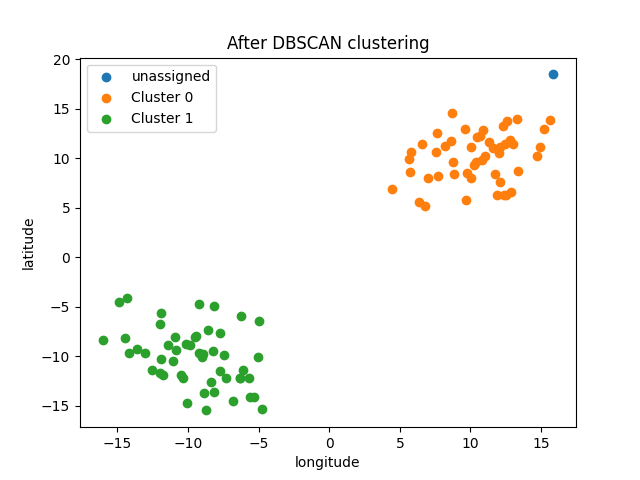
\includegraphics[width=\textwidth]{GPS_clustering_5.png}      
    \end{subfigure}
    \caption{DBSCAN 예시}
  \end{figure}
  오른쪽의 클러스터1에서 다소 떨어져 있는 데이터 하나를 클러스터에 할당하지 않은 모습입니다.
  이처럼 noise를 인식할 수 있고, 클러스터의 개수를 미리 정하지 않아도 된다는 점이 큰 장점입니다.

  \subsection{코드 설명}
  \subsubsection{Classifier.DBSCAN}
  label\_counter는 현재 몇 번째 클러스터를 작업하고 있는지를 나타냅니다.
  클러스터의 index는 0부터 시작이니 처음엔 label\_counter는 0으로 초기화합니다.
  또한 클러스터링 결과를 담는 label도 처음엔 모두 noise를 나타내는 -1로 초기화합니다.
  \begin{python}[label={GPS_clustering_5}]
    label_counter = 0
    label = np.array([-1] * (data.size // 2))
  \end{python}
  주어진 rad와 thres를 이용하여 code data와 noise를 구분합니다.
  distance<rad는 rad이하의 거리를 가지는 데이터는 1 아니면 0을 반환합니다.
  따라서 np.sum(distance<rad,axis=1)는 각 데이터의 반경 rad이하의 거리에 몇 개의 데이터가 있는지 구합니다.
  np.sum(distance < rad, axis=1) >= thres는 위에서 구한 것이 thres 이상인 것들의 index를 구하고 이것이 core data의 index가 됩니다.
  noise의 경우, 반대로 위에서 구한 것이 thres 미만인 것들이니 부등호를 반대로 하여 구합니다.
  \begin{python}[label={GPS_clustering_6}]
    distance = np.array([np.linalg.norm(data - c, axis=1) for c in data])
    core_data = np.sum(distance < rad, axis=1) >= thres
    noise = np.sum(distance < rad, axis=1) < thres
  \end{python}
  core data의 할당을 위해 unassigned\_data에 아직 할당되지 않은 core data의 index를 기록하고,
  첫 클러스터에 첫 번째 할당되지 않은 데이터의 index를 넣습니다.
  \begin{python}[label={GPS_clustering_7}]
    unassigned_data = np.where(core_data == True)[0]
    cluster = np.array([unassigned_data[0]])
  \end{python}
  unassigned\_data가 없을 때까지, 클러스터를 위에서 소개한 방법으로 확장하고 label에 클러스터 할당을 기록하고 label\_counter를 1 증가시키고 cluster를 첫번째 할당하지 않은 데이터로 만들어 다음 클러스터를 할당할 수 있게 준비합니다.
  클러스터의 확장은 self.\_\_extend\_clusters 메소드를 사용했으며, 이는 클러스터에 들어간 데이터의 index가 담긴 list를 반환합니다.
  \begin{python}[label={GPS_clustering_8}]
    while True:
      cluster = self.__extend_cluster(data, cluster, unassigned_data, rad, thres)
      label[cluster] = label_counter
      label_counter += 1
      unassigned_data = np.setdiff1d(unassigned_data, cluster)
      if unassigned_data.size == 0:
        break
      cluster = np.array([unassigned_data[0]])
  \end{python}
  noise의 할당을 위해 unassigned\_data에 noise 데이터의 index를 넣습니다.
  i는 현재 i번째 unassigned\_data에서 할당이 이뤄지고 있음을 의미합니다.
  \begin{python}[label={GPS_clustering_9}]
    unassigned_data = np.where(noise == True)[0]
    i = 0
  \end{python}
  current\_i에 현재 할당 중인 데이터의 원래 index를 저장합니다.
  neighbor에서 current\_i의 index를 가지는 데이터와 거리가 0 초과 rad 미만인 데이터의 index를 구합니다.
  neighbor를 거리가 작은 순으로 정렬하여 nearest를 만듭니다.
  짧은 거리를 가진 데이터부터 살펴, 만약 그 데이터가 noise라면 넘어갑니다.
  만약 그 데이터가 이미 할당된 데이터라면 같은 클러스터에 현재의 noise 데이터를 할당하고 다음 unassigned\_data로 넘어갑니다.
  모든 unassigned\_data에 대해 이 과정을 거쳐 할당할 수 있는 noise는 모두 할당합니다.
  \begin{python}[label={GPS_clustering_10}]
    while i < len(unassigned_data):
      current_i = unassigned_data[i]
      neighbor = np.where(
        (distance[current_i] < rad) & (0 < distance[current_i])
      )[0]
      nearest = np.argsort(distance[current_i][neighbor])
      for j in nearest:
        if label[neighbor[j]] == -1:
          continue
        label[current_i] = label[neighbor[j]]
        break
      i += 1
  \end{python}
  완성된 Label을 반환합니다.
  \begin{python}[label={GPS_clustering_11}]
    return Label
  \end{python}

  \subsubsection{Classifier.\_\_extend\_cluster}
  i는 현재 작업중인 cluster argument에 포함된 데이터의 index입니다.
  처음엔 0으로 초기화하고 cluster.size와 같아지면, 모든 cluster에 포함된 데이터에 대해 확장을 시도했다는 것을 의미합니다.
  \begin{python}[label={GPS_clustering_12}]
    i=0    
  \end{python}
  current\_point에는 원래 데이터의 index가 저장됩니다.
  distance는 원래 데이터와 unassigned\_data 사이의 거리가 저장됩니다.
  neighbor에는 unassigned\_data 중 원래 데이터와 거리가 rad 미만인 것의 index가 저장됩니다.
  만약, neighbor가 빈 list가 아니면 neighbor에 있는 index를 모두 cluster에 합집합으로 추가합니다.
  또한, unassigned\_data에서 추가된 데이터를 차집합하여 제거합니다.
  그 후, cluster의 다음 데이터로 넘어가 cluster 확장과정을 반복합니다.
  \begin{python}[label={GPS_clustering_13}]
    while i < cluster.size:
      current_point = cluster[i]
      distance = np.linalg.norm(
        data[unassigned_data] - data[current_point], axis=1
      )
      neighbor = unassigned_data[np.where(distance < rad)[0]]
      if neighbor.size != 0:
        cluster = np.union1d(cluster, neighbor)
        unassigned_data = np.setdiff1d(unassigned_data, neighbor)
      i += 1
  \end{python}
  확장된 cluster를 반환합니다.
  \begin{python}[label={GPS_clustering_14}]
    return cluster    
  \end{python}

  \section{self.adaptive\_k\_mean}
  \subsection{이론 설명}
  GPS 피쳐를 구할 때 참고한 Sohrab\cite{Sohrab}에서 adaptive-k-mean clustering 알고리즘을 사용했다고 소개하고 있다.
  adaptive-k-mean clustering에 대해 찾아보니 논문마다 조금씩 알고리즘이 다른 것 같았다.
  본 코드는 Sanjiv\cite{Sanjiv}를 참고하여 구현하였다.
  Sanjiv\cite{Sanjiv}에서 소개하는 adaptive-k-mean clustering 알고리즘은 다음과 같다.
  \paragraph{Adaptive-k-mean clustering 알고리즘}
  \begin{enumerate}
    \item 먼저, 클러스터의 개수 k를 정한다.
    \item 데이터에서 랜덤으로 k개를 k개의 클러스터에 할당합니다.
    \item 각 클러스터의 centroid와 클러스터 사이의 최소거리인 d를 구합니다.
    \item 할당되지 않은 데이터와 각 centroid 사이의 거리를 구해 그 최소거리를 d'으로 합니다.
    \item 만약 d'이 d보다 작으면 해당하는 클러스터에 할당합니다.
    \item 만약 d'이 d보다 크면 최소거리 d를 가진 두 클러스터를 합쳐 하나의 클러스터로 만들고 현재 데이터를 하나의 데이터를 가지는 하나의 새로운 클러스터로 만듭니다.
    \item 모든 데이터가 할당될 때까지 앞의 네 단계를 반복합니다.
  \end{enumerate}
  k-mean clustering 알고리즘처럼 미리 클러스터의 개수를 정하고 분류를 한다는 점에서 DBSCAN clustering 알고리즘에 비해 GPS 데이터를 clustering하기에 부적합합니다.
  또한, outlier에 영향을 많이 받는 clustering인데 GPS 데이터는 이동경로라는 outlier가 존재할 수 밖에 없는 데이터라서 더욱 적합하지 않습니다.

  \subsection{예시: Adaptive\_k\_mean.py}
  다음은 클러스터1($\mu_1=\begin{pmatrix}1\\1\end{pmatrix},\sigma_1=\begin{pmatrix}1&0\\0&1\end{pmatrix}$)과
  클러스터2($\mu_2=\begin{pmatrix}-1\\-1\end{pmatrix},\sigma_2=\begin{pmatrix}1&0\\0&1\end{pmatrix}$)에서
  각각 데이터를 50개씩 만들어 $k=2$로 Adaptive-k-mean clustering을 해본 결과입니다.
  \begin{figure}[H]
    \begin{subfigure}[b]{.5\textwidth}
      \centering
      \caption{Before Adaptive-k-mean clustering}
      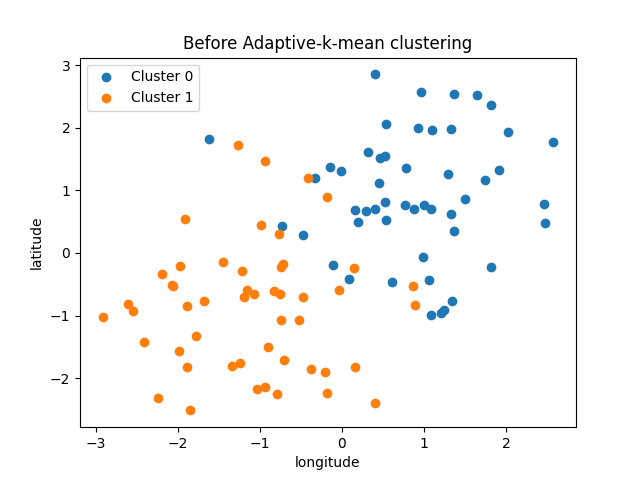
\includegraphics[width=\textwidth]{GPS_clustering_6.png}      
    \end{subfigure}%
    \begin{subfigure}[b]{.5\textwidth}
      \centering
      \caption{After Adaptive-k-mean clustering}
      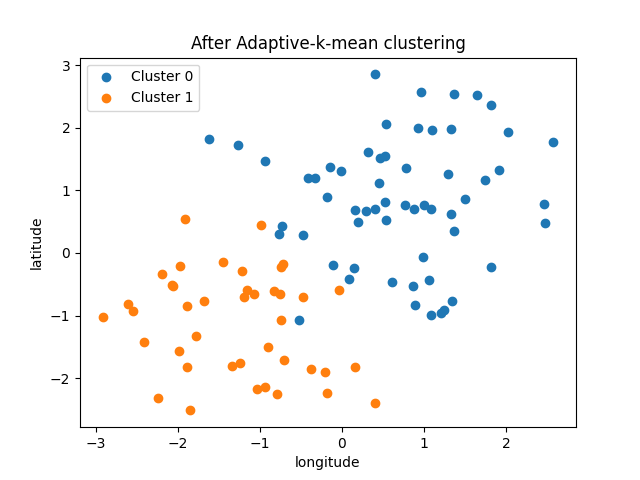
\includegraphics[width=\textwidth]{GPS_clustering_7.png}
    \end{subfigure}
    \caption{Adaptive-k-mean 예시}
  \end{figure}
  k-mean clustering과 달리 산재된 데이터를 유사하게 추정할 수 있습니다.

  \subsection{코드 설명}
  데이터의 개수를 nrow에 저장합니다.
  \begin{python}[label={GPS_clustering_15}]
    nrow = data.shape[0]
  \end{python}
  처음 k개의 데이터를 각각 k개의 클러스터에 할당합니다. 
  seed 리스트의 i번째 원소는 i번째 클러스터에 할당된 데이터의 index입니다.
  \begin{python}[label={GPS_clustering_16}]
    seed = np.random.choice(np.arange(nrow), k, replace=False)
  \end{python}
  처음 label을 모두 -1의 할당되지 않은 상태로 초기화합니다.
  \begin{python}[label={GPS_clustering_17}]
    label = np.array([-1] * nrow)
  \end{python}
  label에 첫 k개의 할당된 데이터를 저장합니다.
  \begin{python}[label={GPS_clustering_18}]
    label[seed] = np.arange(k)
  \end{python}
  각 클러스터마다 데이터가 1개씩 할당되었으니 centroid를 그 데이터로 합니다.
  \begin{python}[label={GPS_clustering_19}]
    centroid = data[seed]
  \end{python}
  각 centroid사이의 거리를 구해 distance에 저장합니다.
  \begin{python}[label={GPS_clustering_20}]
    cluster_dis = np.array([np.linalg.norm(centroid - c, axis=1) for c in centroid])
  \end{python}
  distance에서 자기 자신과의 거리는 고려하지 않기 위해 무한대로 설정합니다.
  \begin{python}[label={GPS_clustering_21}]
    np.fill_diagonal(cluster_dis, np.inf)
  \end{python}
  클러스터 사이의 최소 거리 d를 cluster\_min\_dis에 저장합니다.
  \begin{python}[label={GPS_clustering_22}]
    cluster_min_dis = np.min(cluster_dis)
  \end{python}
  최소 거리 d가 되는 두 클러스터의 index를 closest\_clusters에 저장합니다.
  \begin{python}[label={GPS_clustering_23}]
    closest_clusters = np.unravel_index(cluster_dis.argmin(), cluster_dis.shape)
  \end{python}
  label를 앞에서부터 돌아보며 할당되었다면 넘어갑니다.
  할당되지 않았다면 centroid와의 거리를 to\_cluster\_dis에 저장합니다.
  np.min(to\_cluster\_dis)은 d'을 의미합니다.
  만약 d'이 d이하라면 가장 가까운 centroid의 클러스터로 데이터를 할당하고 centroid를 갱신합니다.
  만약 d'이 d초과라면 d의 거리를 가지는 두 클러스터의 index가 담긴 closest\_clusters의 첫번째 index로 두 클러스터를 합치고, 두번째 index로 현재의 데이터를 할당합니다.
  그 후, 합쳐진 클러스터와 새로 현재의 데이터가 할당된 클러스터의 centroid를 갱신합니다.
  두 경우에서 모두 cluster\_dis, cluster\_min\_dis, closest\_clusters는 갱신함으로 조건문 뒤에 따로 붙혀 줍니다.
  \begin{python}[label={GPS_clustering_24}]
    for i in range(nrow):
      if label[i] != -1:
          continue
      to_cluster_dis = np.array([np.linalg.norm(data[i] - c) for c in centroid])
      if np.min(to_cluster_dis) <= cluster_min_dis:
          updated_cluster = np.argmin(to_cluster_dis)
          label[i] = updated_cluster
          centroid[updated_cluster] = np.mean(data[label == updated_cluster])
      else:
          merged_cluster = closest_clusters[0]
          new_cluster = closest_clusters[1]
          label[label == new_cluster] = merged_cluster
          label[i] = new_cluster
          centroid[merged_cluster] = np.mean(data[label == merged_cluster])
          centroid[new_cluster] = data[i]
      cluster_dis = np.array(
          [np.linalg.norm(centroid - c, axis=1) for c in centroid]
      )
      np.fill_diagonal(cluster_dis, np.inf)
      cluster_min_dis = np.min(cluster_dis)
      closest_clusters = np.unravel_index(cluster_dis.argmin(), cluster_dis.shape)
  \end{python}
  완성된 label을 반환합니다.
  \begin{python}[label={GPS_clustering_25}]
    return label    
  \end{python}

  \section{self.neighbor}
  \subsection{이론 설명}
  neighbor clustering은 단순히 주어진 point에서 rad이하의 거리에 있는 점들을 고르는 clustering입니다.
  GPS 피쳐 중, Home\_stay 같은 것들은 주어진 점 근처에 있는 데이터를 고르는 것이 필요하여 구현했습니다.

  \subsection{예시: Neighbor.py}
  다음은 $\mu=\begin{pmatrix}0\\0\end{pmatrix},\sigma=\begin{pmatrix}1&0\\0&1\end{pmatrix}$인 클러스터에서 데이터 100개를 만들어 $point=\begin{pmatrix}0\\0\end{pmatrix},rad=1$로 neighbor clustering한 결과입니다.
  \begin{figure}[H]
    \begin{subfigure}[b]{.5\textwidth}
      \centering
      \caption{Before neighbor clustering}
      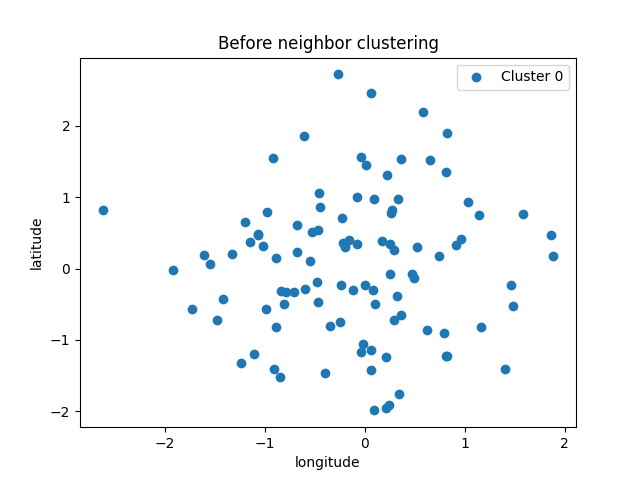
\includegraphics[width=\textwidth]{GPS_clustering_8.png}      
    \end{subfigure}%
    \begin{subfigure}[b]{.5\textwidth}
      \centering
      \caption{After neighbor clustering}
      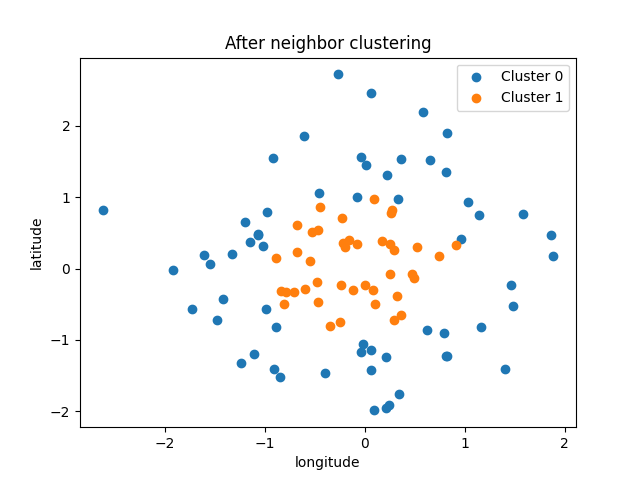
\includegraphics[width=\textwidth]{GPS_clustering_9.png}
    \end{subfigure}
    \caption{Neighbor 예시}
  \end{figure}

  \subsection{코드 설명}
  주어진 point와 거리 rad이하에 있는 데이터의 index를 반환합니다.
  \begin{python}[label={GPS_clustering_26}]
    return (np.linalg.norm(data - point, axis=1) <= rad).astype(int)
  \end{python}

  \chapter{GPS\_feature}
  \setcounter{section}{0}
  \section{데이터 수집}
  GPS 피쳐는 오차에 민감한 경우도 있습니다. 따라서 preprocess를 거쳐 오차를 보정한 data\_smoothed.csv 파일을 Data 파일에 복사해 넣어 사용합니다.
  또한 Label\_dataload에서 만든 label.csv 파일도 Data 파일에 넣어 사용합니다.(Home\_stay와 같은 피쳐의 계산에 필요합니다.)
  \begin{figure}[H]
    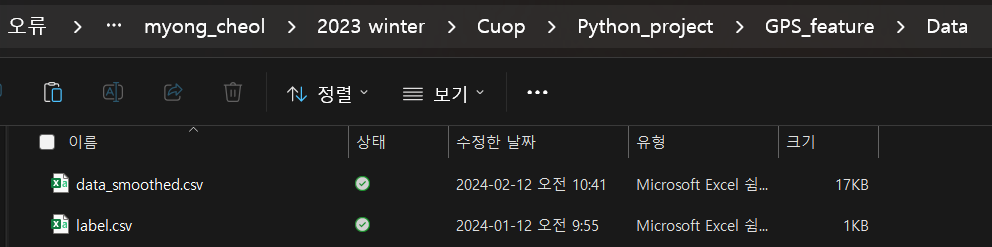
\includegraphics[width=\textwidth]{GPS_feature_1.png}
  \end{figure}

  \section{모듈: GPS\_feature.py}
  modules 폴더를 열어보면 아래와 같이 GPS\_clustering.py와 GPS\_feature.py의 두 모듈이 있는 것을 확인할 수 있습니다.
  GPS\_clustering.py는 ClusterGenerator, Classifier의 두 클래스로 구성되어 있습니다.
  \begin{figure}[H]
    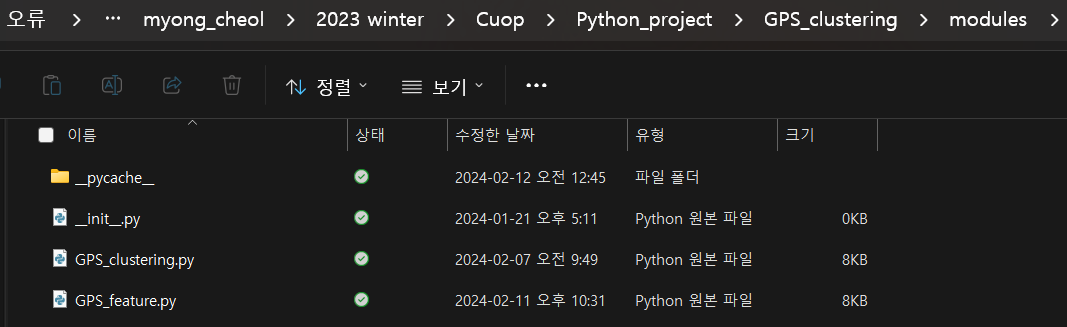
\includegraphics[width=\textwidth]{GPS_clustering_1.png}
  \end{figure}
  \subsection{클래스: FeatureMaker}
  FeatureMaker 클래스의 구조는 다음과 같습니다.
  \dirtree{%
  .0 GPS\_feature.py.
  .1 class: FeatureMaker.
  .2 method: self.\_\_init\_\_.
  .2 method: self.location\_variance.
  .2 method: self.total\_distance.
  .2 method: self.speed.
  .2 method: self.speed\_mean.
  .2 method: self.speed\_variance.
  .2 method: self.number\_of\_clusters.
  .2 method: self.\_\_time.
  .2 method: self.entropy.
  .2 method: self.normalized\_entropy.
  .2 method: self.home\_stay.
  .2 method: self.transition\_time.
  .2 method: self.circadian\_movement.
  .2 method: self.harversine.
  .2 method: self.activity\_percentile.
  }
  GPS\_feature.py 모듈은 클래스 FeatureMaker 하나로 이루어져 있습니다.
  본 모듈이 계산하는 피쳐들은 Sohrab\cite{Sohrab}에 소개되어 있습니다.
  FeatureMaker에서는 다양한 피쳐를 계산하는 메소드와 그 메소드를 보조하는 메소드로 구성되었습니다.
  self.\_\_init\_\_에서는 rad, thres, home\_rad attributes를 초기화합니다. 
  rad, thres는 피쳐계산시 수행하는 DBSCAN clustering을 할 때 사용합니다.
  home\_rad는 Home\_stay 피쳐를 계산할 때 사용합니다.
  다른 메소드에 대한 설명은 아래에 있습니다.

  \section{사용법: GPS\_feature\_test.py}
  GPS\_feature\_test.py를 실행하면, GPS\_feature\textbackslash Feature파일에 feature.csv가 만들어진 것을 확인할 수 있습니다.
  이는 data\_smoothed.csv 파일과 label.csv 파일을 읽어 계산한 피쳐를 저장한 파일입니다.
  \begin{figure}[H]
    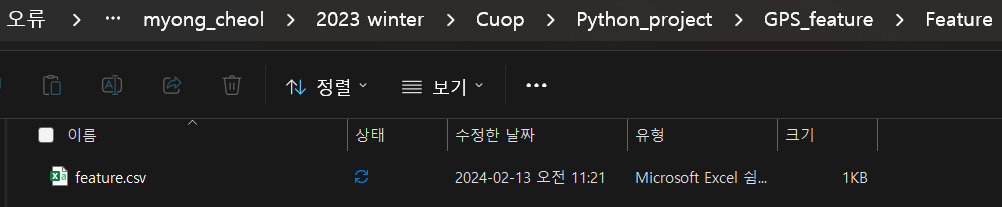
\includegraphics[width=\textwidth]{GPS_feature_2.png}
  \end{figure}
  또한, GPS\_feature\textbackslash Plot파일에 피쳐계산과 관련된 여러 가지 사진들이 있는 것을 볼 수 있습니다.
  \begin{figure}[H]
    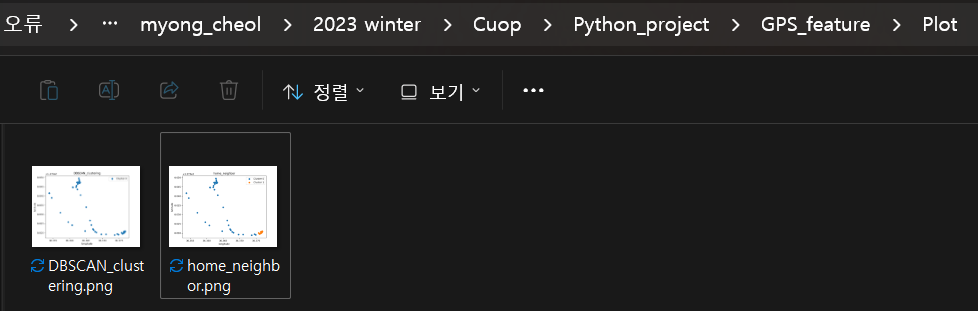
\includegraphics[width=\textwidth]{GPS_feature_3.png}
  \end{figure}

  \section{self.location\_variance}
  \subsection{이론 설명}
  Sohrab\cite{Sohrab}에서는 다음과 같이 location\_variance를 정의하고 있습니다.
  \[location\_variance=\log(\sigma_{lat}^2+\sigma_{long}^2)\]
  여기서 $\sigma_{lat}^2$, $\sigma_{long}^2$는 latitude, longitude의 분산을 의미합니다.
  이 정의를 그대로 이용하여 코드를 구현했습니다.

  \subsection{예시: GPS\_feature\_test.py}
  FeatureMaker 클래스의 인스턴스를 생성후, 아래와 같이 사용할 수 있습니다.
  \begin{python}[label={GPS_feature_1}]
    location_variance = featuremaker.location_variance(data)
  \end{python}

  \subsection{코드 설명}
  longitude, latitude의 분산을 구해 longitude\_variance, latitude\_variance에 저장합니다.
  \begin{python}[label={GPS_feature_2}]
    longitude_variance = data["longitude"].std()
    latitude_variance = data["latitude"].std()
  \end{python}
  두 분산을 더해 로그를 취하여 반환합니다.
  \begin{python}[label={GPS_feature_3}]
    return np.log2(longitude_variance + latitude_variance)
  \end{python}

  \section{self.total\_distance}
  \subsection{이론 설명}
  Sohrab\cite{Sohrab}에서는 다음과 같이 total\_distance를 정의하고 있습니다.
  \[total\_distance=\sum_i{\sqrt{(lat_i-lat_{i-1})^2+(long_i-long_{i-1})^2}}\]
  이 정의를 그대로 이용하여 코드를 구현했습니다.

  \subsection{예시: GPS\_feature\_test.py}
  FeatureMaker 클래스의 인스턴스를 생성한 후, 아래와 같이 사용할 수 있습니다.
  \begin{python}[label={GPS_feature_4}]
    total_distance = featuremaker.total_distance(data)
  \end{python}

  \subsection{코드 설명}
  latitude와 longitude의 연속된 두 점의 차이를 diff\_latitude, diff\_longitude에 저장합니다.
  \begin{python}[label={GPS_feature_5}]
    diff_longitude = (data["longitude"].diff()).iloc[1:]
    diff_latitude = (data["latitude"].diff()).iloc[1:]
  \end{python}
  diff\_latitude와 diff\_longitude를 제곱하여 더한 후, 제곱근을 취해 다 더합니다.
  \begin{python}[label={GPS_feature_6}]
    return np.sum(np.sqrt(np.square(diff_longitude) + np.square(diff_latitude)))
  \end{python}

  \section{self.speed, self.speed\_mean, self.speed\_variance}
  \subsection{이론 설명}
  Sohrab\cite{Sohrab}에서는 speed를 다음과 같이 정의하고 있습니다.
  \[speed_i=\sqrt{(\frac{lat_i-lat_{i-1}}{t_i-t_{i-1}})^2+(\frac{long_i-long_{i-1}}{t_i-t_{i-1}})^2}\]
  이 정의를 그대로 이용하여 코드를 구현했습니다.

  \subsection{예시: GPS\_feature\_test.py}
  FeatureMaker 클래스의 인스턴스를 생성한 후, 아래와 같이 사용할 수 있습니다.
  \begin{python}[label={GPS_feature_7}]
    speed_variance = featuremaker.speed_variance(data)
    speed_mean = featuremaker.speed_mean(data)
  \end{python}

  \subsection{코드 설명}
  \subsubsection{코드 설명: self.speed}
  latitude와 longitude, obtained\_at의 연속된 두 점의 차이를 diff\_latitude, diff\_longitude, diff\_time에 저장합니다.
  이 때 diff\_time의 단위는 초가 되도록 단위를 변환해줍니다.
  \begin{python}[label={GPS_featue_8}]
    diff_longitude = (data["longitude"].diff()).iloc[1:]
    diff_latitude = (data["latitude"].diff()).iloc[1:]
    diff_time = (data["obtained_at"].diff()).iloc[1:] / pd.Timedelta(seconds=1)
  \end{python}
  정의된 수식에 따라 speed를 계산하여 반환합니다.
  \begin{python}[label={GPS_feature_9}]
    return np.sqrt(
      np.square(diff_longitude / diff_time) + np.square(diff_latitude / diff_time)
    )
  \end{python}

  \subsubsection{코드 설명: self.speed\_mean}
  self.speed로 speed를 구하고 이것의 평균을 반환합니다.
  \begin{python}[label={GPS_feature_10}]
    return np.mean(self.speed(data))
  \end{python}

  \subsubsection{코드 설명: self.speed\_variance}
  self.speed로 speed를 구하고 이것의 분산을 반환합니다.
  \begin{python}[label={GPS_feature_11}]
    return np.std(self.speed(data))
  \end{python}

  \section{self.number\_of\_clusters}
  \subsection{이론 설명}
  Sohrab\cite{Sohrab}에서는 number\_of\_clusters를 구하기 위해 adaptive-k-mean clustering을 사용했다고 소개합니다.
  그러나, 상기한 단점들로 인해 저는 DBSCAN clustering을 사용하여 구하기로 결정했습니다.
  아래는 제 1월 17일 데이터를 preprocess를 거친 다음, $rad=0.002,thres=5$로 DBSCAN clustering한 결과입니다.
  \begin{figure}[H]
    \centering
    \caption{ DBSCAN clustering: 2024/1/17}
    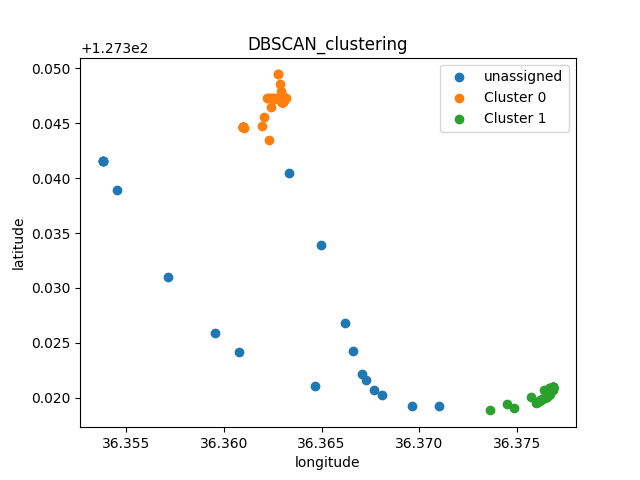
\includegraphics[width=.5\textwidth]{GPS_feature_4.png}
  \end{figure}

  \subsection{예시: GPS\_feature\_test.py}
  FeatureMaker 클래스의 인스턴스를 생성한 후, 아래와 같이 사용할 수 있습니다.
  \begin{python}[label={GPS_feature_12}]
    number_of_clusters = featuremaker.number_of_clusters(data)
  \end{python}

  \subsection{코드 설명}
  먼저, FeatureMaker 클래스의 인스턴스 featuremaker를 생성합니다.
  \begin{python}[label={GPS_feature_13}]
    classifier = Classifier()
  \end{python}
  classifier의 DBSCAN 메소드를 사용하기 위해 데이터를 numpy array로 변환합니다.
  \begin{python}[label={GPS_feature_14}]
    np_data = data[["latitude", "longitude"]].to_numpy()
  \end{python}
  classifier의 DBSCAN 메소드를 사용하여 clustering한 label을 얻습니다.
  \begin{python}[label={GPS_feature_15}]
    label = classifier.DBSCAN(np_data, self.rad, self.thres)
  \end{python}  
  클러스터의 index는 0부터 시작함으로, 전체 클러스터의 수는 label의 최대치 더하기 1입니다.
  따라서 이를 반환합니다.
  \begin{python}[label={GPS_feature_16}]
    return np.max(label) + 1
  \end{python}

  \section{self.\_\_time, self.entropy, self.normalized\_entropy}
  \subsection{이론 설명}
  Sohrab\cite{Sohrab}에서 entropy와 normalized\_entropy를 다음과 같이 정의하고 있습니다.
  \[entropy=-\sum_{i=1}^N{p_i\log p_i},normalized\_entropy=\frac{entropy}{\log N}\]
  여기서 $p_i$는 i번째 장소에서 쓴 시간의 퍼센트입니다.
  이 정의를 그대로 이용하여 코드를 구현했습니다.
  방문한 장소의 경우, DBSCAN clustering으로 구했습니다.
  self.\_\_time에서 $p_i$를 구하고 다른 메소드에서 각각 원하는 피쳐를 계산합니다.

  \subsection{예시: GPS\_feature\_test.py}
  FeatureMaker 클래스의 인스턴스를 만든 후, 아래와 같이 사용할 수 있습니다.
  \begin{python}[label={GPS_feature_17}]
    entropy = featuremaker.entropy(data)
    normalized_entropy = featuremaker.normalized_entropy(data)
  \end{python}

  \subsection{코드 설명}
  \subsubsection{self.\_\_time}
  클러스터의 개수를 N에 저장합니다. 또한 각 클러스터에서 머무른 시간을 저장할 time\_list도 만듭니다.
  \begin{python}[label={GPS_feature_18}]
    N = np.max(label) + 1
    time_list = np.array([])
  \end{python}
  index에 i번째 클러스터를 구성하고 있는 데이터의 index를 저장합니다.
  그리고 index에 원래 데이터의 마지막 index가 있다면 제거해 줍니다.
  i번째 클러스터에 머문 시간을 time에 저장합니다. 그 후, time을 time\_list에 넣어줍니다.
  이 과정을 모든 클러스터에 대해 반복합니다.
  \begin{python}[label={GPS_feature_19}]
    for i in range(N):
      index = np.where(label == i)[0]
      index = np.setdiff1d(index, np.array([len(label) - 1]))
      time = np.sum(
          np.diff(data["obtained_at"].to_numpy())[index] / pd.Timedelta(seconds=1)
      )
      time_list = np.append(time_list, [time])
  \end{python}
  time\_list를 time\_list에 들어있는 시간의 합으로 나누어 각 클러스터에서 머둔 시간의 퍼센트를 구한 후, 반환합니다.
  \begin{python}[label={GPS_feature_20}]
    return time_list / np.sum(time_list)
  \end{python}

  \subsubsection{self.entropy}
  DBSCAN clustering을 하기 위해 Classifier 클래스의 인스턴스 classifier를 생성합니다.
  \begin{python}[label={GPS_feature_21}]
    classifier = Classifier()
  \end{python}
  classifier의 DBSCAN 메소드에 넣을 data를 numpy array로 변환시켜 np\_data에 저장합니다.
  \begin{python}[label={GPS_feature_22}]
    np_data = data[["latitude", "longitude"]].to_numpy()
  \end{python}
  DBSCAN clustering을 수행하고 그 결과를 label에 저장합니다.
  \begin{python}[label={GPS_feature_23}]
    label = classifier.DBSCAN(np_data, self.rad, self.thres)
  \end{python}
  self.\_\_time 메소드를 사용해 각 클러스터에서 머문 시간의 퍼센트를 percentage에 저장합니다.
  \begin{python}[label={GPS_feature_24}]
    percentage = self.__time(data, label)
  \end{python}
  entropy 공식에 따라 entropy를 계산하여 반환합니다.
  \begin{python}[label={GPS_feature_25}]
    return -np.sum(percentage * np.log2(percentage))
  \end{python}

  \subsubsection{self.normalized\_entropy}
  각 클러스터에서 머문 시간의 퍼센트를 percentage에 저장하는 부분까지 이전과 같습니다.
  \begin{python}[label={GPS_feature_26}]
    classifier = Classifier()
    np_data = data[["latitude", "longitude"]].to_numpy()
    label = classifier.DBSCAN(np_data, self.rad, self.thres)
    percentage = self.__time(data, label)
  \end{python}
  normalized\_entropy의 공식에 따라 normalized\_entropy를 계산하여 반환합니다.
  \begin{python}[label={GPS_feature_27}]
    return -np.sum(percentage * np.log2(percentage)) / np.log2(len(percentage))
  \end{python}

  \section{self.home\_stay, self.transition\_time}
  \subsection{이론 설명}
  Sohrab\cite{Sohrab}에서는 home\_stay를 집에 머무른 시간의 퍼센트로 정의하고 있습니다.
  집의 위치에서 반경 rad안에 있는 것들로 clustering할 수 있는 Classifier 클래스의 neighbor 메소드를 사용하여 집에 머무는 점을 구분했습니다.
  아래는 제 1월 17일 데이터를 preprocess를 거친 다음, $home\_rad=0.002$로 neighbor clustering한 결과입니다.
  \begin{figure}[H]
    \centering
    \caption{neighbor clustering: 2024/01/17}
    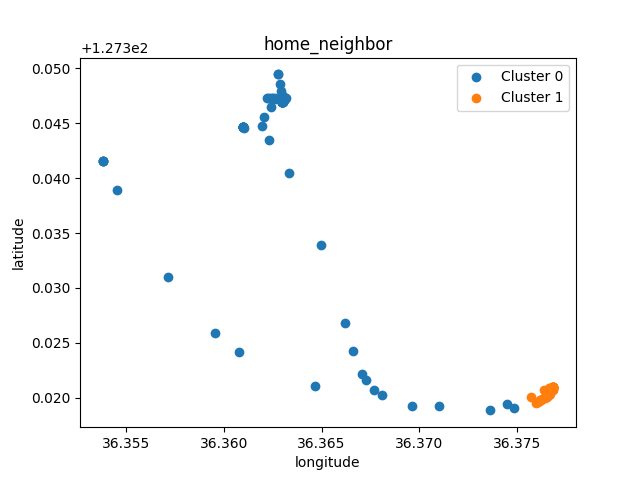
\includegraphics[width=.5\textwidth]{GPS_feature_5.png}
  \end{figure}
  Sohrab\cite{Sohrab}에서는 transition\_time을 교통수단을 이용한 시간의 퍼센트로 정의하고 있습니다.
  저는 DBSCAN clustering으로 할당되지 않은 데이터들을 머물러 있지 않는 데이터, 즉 교통수단을 이용한 데이터로 판단하여 사용했습니다.

  \subsection{예시: GPS\_feature\_test.py}
  FeatureMaker 클래스의 인스턴스 featuremaker를 생성한 후, 아래와 같이 사용할 수 있습니다.
  home\_label의 경우, label.csv에서 name 컬럼이 Home인 것을 뽑아 구합니다.
  \begin{python}[label={GPS_feature_28}]
    home_stay = featuremaker.home_stay(data, home_label=home_label)
    transition_time = featuremaker.transition_time(data)
  \end{python}

  \subsection{코드 설명}
  \subsubsection{self.home\_stay}
  home\_label에서 집의 위치정보만 뽑아 home\_location에 numpy arrary로 저장합니다.
  \begin{python}[labe={GPS_feature_29}]
    home_location = home_label[["latitude", "longitude"]].to_numpy()
  \end{python}
  Classifier 클래스의 인스턴스 classifier를 만들고 neighbor clustering을 수행해, 그 결과를 label에 저장합니다.
  \begin{python}[label={GPS_feature_30}]
    classifier = Classifier()
    np_data = data[["latitude", "longitude"]].to_numpy()
    label = classifier.neighbor(np_data, home_location, self.home_rad)
  \end{python}
  label이 1이면 집 근처에 있었다는 의미입니다. 따라서 그런 데이터의 index를 모아 home\_index에 저장합니다.
  \begin{python}[label={GPS_fearue_31}]
    home_index = np.where(label == 1)[0]
  \end{python}
  각 데이터 별, 그 위치에 머문 시간을 diff\_time에 초 단위로 저장합니다.
  \begin{python}[label={GPS_feature_32}]
    diff_time = (data["obtained_at"].diff()).iloc[1:].reset_index(
        drop=True
    ) / pd.Timedelta(seconds=1)
  \end{python}
  만약 home\_index에 원래 데이터의 마지막 index가 있다면 제거합니다.
  왜냐하면 diff를 수행할 때 마지막 index에 해당하는 diff 값은 구할 수 없기 때문입니다. 
  \begin{python}[label={GPS_feature_33}]
    if diff_time.shape[0] <= np.max(home_index):
      home_index = home_index[:-1]
  \end{python}
  하루는 86400초이니, home\_index를 바탕으로 집에 머문 시간을 계산하여 86400으로 나누고 이를 반환합니다.
  \begin{python}[label={GPS_feature_34}]
    return np.sum(diff_time.iloc[home_index]) / 86400
  \end{python}

  \subsubsection{self.transition\_time}
  이전과 home\_label을 다루지 않고 DBSCAN clustering을 사용해 할당되지 않은 -1의 label을 가진 데이터만 고려한다는 점만 다릅니다.
  \begin{python}[label={GPS_feature_35}]
    classifier = Classifier()
    np_data = data[["latitude", "longitude"]].to_numpy()
    label = classifier.DBSCAN(np_data, self.rad, self.thres)
    transition_index = np.where(label == -1)[0]
    diff_time = (data["obtained_at"].diff()).iloc[1:].reset_index(
        drop=True
    ) / pd.Timedelta(seconds=1)
    if diff_time.shape[0] <= np.max(transition_index):
        transition_index = transition_index[:-1]
    return np.sum(diff_time[transition_index]) / 86400
  \end{python}

  \section{self.circadian\_movement}
  \subsection{이론 설명}
  \begin{definition}[푸리에 급수]
    주기함수 $f:\mathbb{R}\to\mathbb{C}$가 주기 T를 가진다고 하자. 즉, $f(x)=f(x+T)$이라고 하자.
    또한, $f$가 모든 유한 구간에서 제곱적분 가능하다고 하자. 즉, 임의의 $a,b\in\mathbb{R}$에 대해, $\int_{a}^b{\left\vert f\right\vert^2}\,dx$는 유한하다.
    이 때, $f$의 푸리에 계수 $g_n$을 다음과 같이 정의합니다.
    \[g_n=\frac{1}{T}\int_{t_0}^{t_0+T}{\exp(-\frac{2n\pi ix}{T})f(x)}\,dx\]
    그렇다면, $f$의 푸리에 급수는 다음과 같습니다.
    \[f(x)=\sum_{-\infty}^{\infty}{g_n\exp(\frac{2n\pi ix}{T})}\]
  \end{definition}
  즉, 임의의 주기함수를 삼각함수들의 합으로 나타낼 수 있습니다.
  여기서 비주기함수를 주기가 무한대인 함수로 간주하고 푸리에급수를 계산할 수 있습니다.
  Power spectral density는 그렇게 구한 푸리에 계수를 의미합니다.\newline
  Sohrab\cite{Sohrab}에서는 circadian\_movement를 다음과 같이 정의하고 있습니다.
  \[CM=\log(E_{lat}+E_{long}),E=\frac{1}{i_u-i_L}\sum_{i=i_L}^{i_u}{psd(f_i)}\]
  여기서 $psd(f_i)$는 frequency가 $f_i$인 power spectral density입니다.
  또한, $i_L,i_u$는 관심있는 frequency의 lower, upper bound입니다.
  Circadian\_movement를 구하기 위해 23.5에서 24.5시간의 frequency를 가지는 신호에 관심을 가지고 있습니다.

  \subsection{예시: Circadian\_movement.py}
  제 2023년 12월 한 달의 raw data를 이용하여 circadian movement를 구해봤습니다.
  먼저, raw data의 latitude와 longitude를 그려봤습니다.
  \begin{figure}[H]
    \begin{subfigure}[b]{.5\textwidth}
      \centering
      \caption{2023/12 latitude}
      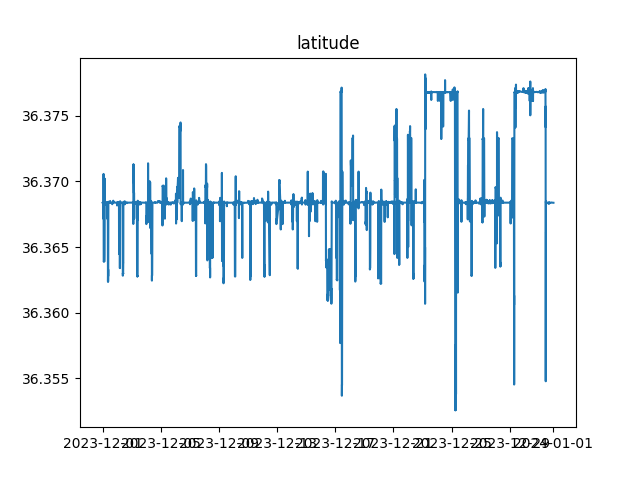
\includegraphics[width=\textwidth]{GPS_feature_6.png}
    \end{subfigure}%
    \begin{subfigure}[b]{.5\textwidth}
      \centering
      \caption{2023/12 longitude}
      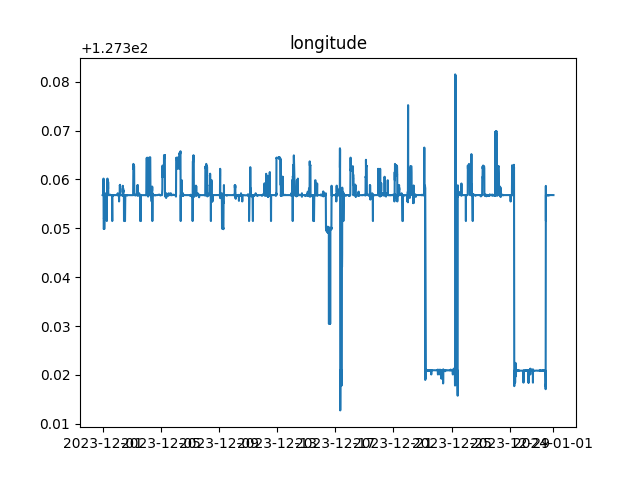
\includegraphics[width=\textwidth]{GPS_feature_7.png}
    \end{subfigure}
  \end{figure}
  하루 단위로 주기성을 가지고 있는 것처럼 보입니다.
  이를 이용하여 fft(fast fourier transformation)을 한 결과는 다음과 같습니다.
  \begin{figure}[H]
    \centering
    \caption{fast fourier transformation: 2023/12}
    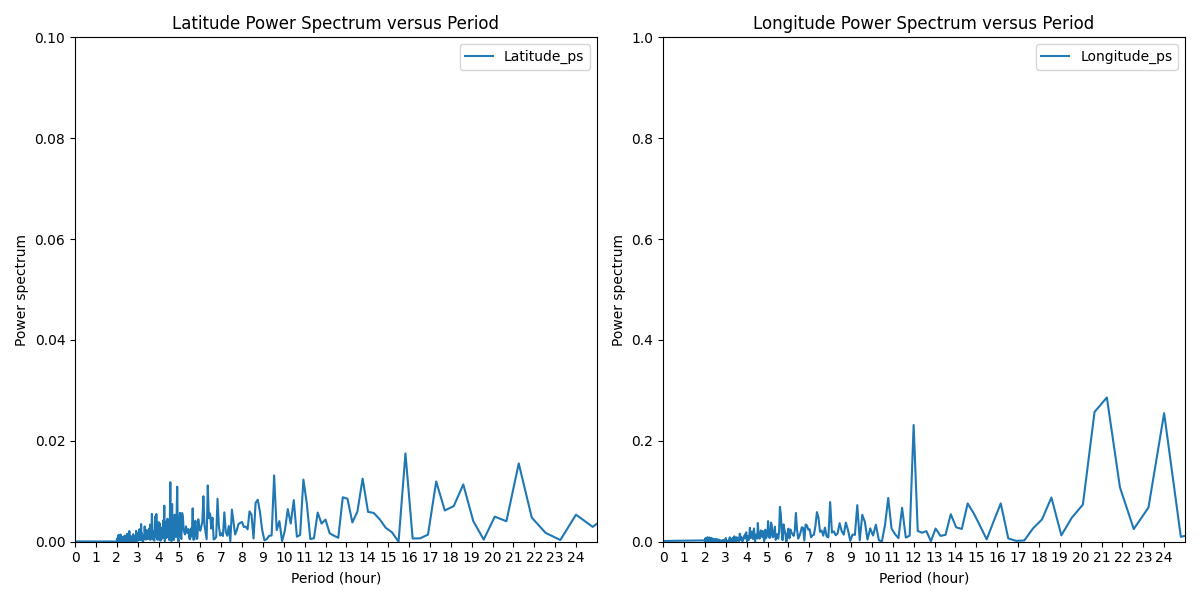
\includegraphics[width=\textwidth]{GPS_feature_8.png}
  \end{figure}
  latitude의 경우 신호가 약해 오차의 영향이 큼으로 분석에서 배제하겠습니다.
  longitude의 경우 12시간과 24시간 언저리에 신호가 있다는 것을 볼 수 있습니다.
  모듈이 반환하는 값은 23.5~24.5시간의 frequency를 가지는 psd의 합에 로그 함수를 취한 것입니다.

  \subsection{코드 설명}
  먼저, raw data를 전처리합니다. 1시간 간격으로 평균을 내어 시간 별로 데이터가 있도록 변환합니다.
  만약, 1시간 동안 데이터 측정이 없었다면 interpolation을 하여 데이터를 채웁니다.
  그 후, 최빈값이 원점인 0에 있도록 latitude, longitude에서 각각의 최빈값을 뺍니다.
  (주기 함수처럼 만들기 위해서 합니다.)
  \begin{python}[label={GPS_feature_36}]
    data["obtained_at"] = pd.to_datetime(data["obtained_at"])
    time_series = data.set_index("obtained_at")
    time_series = time_series.resample(
        "60T"
    ).mean()
    time_series = time_series.interpolate()
    time_series["latitude"] = (
        time_series["latitude"] - time_series["latitude"].median()
    )
    time_series["longitude"] = (
        time_series["longitude"] - time_series["longitude"].median()
    )
  \end{python}
  numpy에 내장된 fft를 사용해 latitude와 longitude 각각에 fft를 합니다.
  결과는 latitude\_fft, longitude\_fft에 각각 저장합니다.
  \begin{python}[label={GPS_feature_37}]
    latitude_fft = np.fft.fft(time_series["latitude"])
    longitude_fft = np.fft.fft(time_series["longitude"])
  \end{python}
  fft한 결과를 이용해 latitude, longitude의 power spectral density를 구해 latitude\_ps, longitude\_ps에 저장합니다.
  \begin{python}[label={GPS_feature_38}]
    latitude_ps = np.abs(latitude_fft) ** 2
    longitude_ps = np.abs(longitude_fft) ** 2
  \end{python}
  numpy의 fft에 내장된 frequency를 얻는 메소드로 frequency들을 frequencies에 저장합니다.
  \begin{python}[label={GPS_feature_39}]
    frequencies = np.fft.fftfreq(len(time_series), 1)
  \end{python}
  주기가 23.5~24.5시간 사이인 power spectral density를 latitude, longitude 각각에 대해 다 더해 E\_latitude, E\_longitude에 저장합니다.
  \begin{python}[label={GPS_feature_40}]
    index_24 = np.where((1 / frequencies >= 23.5) & (1 / frequencies <= 24.5))[0]
    E_latitude = np.sum(latitude_ps[index_24]).astype(float)
    E_longtitude = np.sum(longitude_ps[index_24]).astype(float)
  \end{python}
  Circadian\_movement의 공식에 따라 계산하여 반환합니다.
  \begin{python}[label={GPS_feature_41}]
    return np.log2(E_latitude + E_longtitude)
  \end{python}

  \section{self.harversine, self.activity\_percentile}
  \subsection{이론 설명}
  Congyu\cite{Congyu}에서는 Circadian movement를 구하는 다양한 방법들을 소개하고 있습니다.
  그 중에서 activity percentile를 구하는 방법이 있습니다.
  시간에 따른 누적 이동 거리를 구한 후, 특정 퍼센트를 지날 때의 시간을 구하는 방법입니다.
  \begin{theorem}[harversine formula]
    단위구 위의 두 점 $P_1=(\phi_1,\lambda_1),P_2=(\phi_2,\lambda_2)$ 사이의 거리 d는 다음과 같이 나타난다.
    \[d=2\arcsin(\sqrt{\sin^2(\frac{\phi_2-\phi_1}{2})+\cos\phi_1\cos\phi_2\sin^2(\frac{\lambda_2-\lambda_1}{2})})\]
    여기서 $\phi$는 위도, $\lambda$는 경도를 나타낸다.
  \end{theorem}
  하버사인 공식을 이용하여 누적 이동 거리를 구하고 activity\_percentile을 구할 수 있습니다.

  \subsection{예시: GPS\_feature\_test.py}
  FeatureMaker 클래스의 인스턴스 featuremaker를 생성한 후, 아래와 같이 사용할 수 있습니다.
  두번째 argument인 0.25는 25\%의 누적 이동을 하였을 떄의 시간을 구하라는 뜻입니다.
  보통 25\%, 50\%, 75\%일 때의 시간을 구해, 하루의 주기를 찾습니다.
  \begin{python}[label={GPS_feature_42}]
    activity_percentile = featuremaker.activity_percentile(data, 0.25)
  \end{python}

  \subsection{코드 설명}
  \subsubsection{self.harversine}
  먼저, 지구반지름을 R에 저장합니다.
  \begin{python}[label={GPS_feature_43}]
    R = 6371.0
  \end{python}
  location1, location2에서 각각 lat1, lon1, lat2, lon2를 구합니다.
  \begin{python}[label={GPS_feature_44}]
    lat1, lon1 = np.radians(location1["latitude"]), np.radians(
        location1["longitude"]
    )
    lat2, lon2 = np.radians(location2["latitude"]), np.radians(
        location2["longitude"]
    )
  \end{python}
  공식에 따라 거리를 계산합니다.
  \begin{python}[label={GPS_feature_45}]
    dlon = lon2 - lon1
    dlat = lat2 - lat1
    a = np.sin(dlat / 2) ** 2 + np.cos(lat1) * np.cos(lat2) * np.sin(dlon / 2) ** 2
    c = 2 * np.arcsin(np.sqrt(a))
    distance = R * c
  \end{python}
  거리를 반환합니다.
  \begin{python}[label={GPS_feature_46}]
    return distance
  \end{python}

  \subsection{self.activity\_percentile}
  먼저, 데이터를 전처리합니다. 10분마다 평균을 내어 데이터를 저장합니다.
  만약, 10분 동안 데이터 측정이 없었다면 interpolation해서 데이터를 채웁니다.
  \begin{python}[label={GPS_feature_47}]
    data.loc[:, "obtained_at"] = pd.to_datetime(data["obtained_at"])
    time_series = data.set_index("obtained_at")
    time_series = time_series.resample("10T").mean()
    time_series = time_series.interpolate()
  \end{python}
  하버사인 공식을 이용하여 연속한 데이터 사이의 이동 거리를 구해 distance list에 저장합니다.
  \begin{python}[label={GPS_feature_48}]
    distance = list()
    for i in range(time_series.shape[0]):
        if i == time_series.shape[0] - 1:
            break
        distance.append(
            self.harversine(time_series.iloc[i], time_series.iloc[i + 1])
        )
  \end{python}
  distance를 누적 이동 거리로 만든 후, 이동거리의 총합으로 나눠 activity\_percentile을 구합니다.
  \begin{python}[label={GPS_feature_49}]
    activity_percentile = np.cumsum(distance) / np.sum(distance)
  \end{python}
  주어진 퍼센트 이상의 누적 이동 거리를 움직인 최초의 index를 찾아 index에 저장합니다.
  \begin{python}[label={GPS_feature_50}]
    index = 0
    while True:
        if activity_percentile[index] >= percentile:
            break
        index += 1
  \end{python}
  그 index를 가지는 데이터의 시간을 반환합니다.
  \begin{python}[label={GPS_feature_51}]
    return time_series.index[index]
  \end{python}
  

  \begin{thebibliography}{9}
    \bibitem{Yannick}
    Yannick Roos.
    \textit{Does Your Smartphone “Know” Your Social Life? A Methodological Comparison of Day Reconstruction, Experience Sampling, and Mobile Sensing}
    \bibitem{Morgon}
    Morgon Quinn Ross.
    \textit{The Psychology of Mobile Technology and Daily Mobility}
    \bibitem{Sohrab}
    Sohrab Saeb.
    \textit{The relationship between mobile phone location sensor data and depressive symptom severity}
    \bibitem{Ali}
    Ali Rostami.
    \textit{A Light-Weight Smartphone GPS Error Model for Simulation}
    \bibitem{Schussler}
    Schussler.
    \textit{Processing raw data from global positioning systems without additional information}
    \bibitem{Elmira}
    Elmira Berjisian.
    \textit{Evaluation of map-matching algorithms for smartphone-based active travel data}
    \bibitem{Adam}
    Adam Millard-Ball.
    \textit{Map-matching poor-quality GPS data in urban environments: The pgMapMatch package}
    \bibitem{김소정}
    김소정.
    \textit{군집 노이즈 필터링 기반 이동 궤적 정제 기법}
    \bibitem{Sanjiv}
    Sanjiv K.Bhatia.
    \textit{Adaptive K-Means Clustering}
    \bibitem{Congyu}
    Congyu Wu.
    \textit{Circadian Rhythms are Not Captured Equal: Exploring Circadian Metrics Extracted by Different Computational Methods from Smartphone Accelerometer and GPS Sensors in Daily Life Tracking}
  \end{thebibliography}
\end{document}